\documentclass[fs, footer]{latex4ei}
\usepackage{latex4ei}
\usepackage[european]{circuitikz}

\usepackage{multirow}
\usepackage{kbordermatrix}
\usepackage{tcolorbox}
\usepackage{latexnew}

% UPDATE WITHOUT CLASS CHANGE
% ----------------------------------------------------------------------

% LastPage
\usepackage{lastpage}

% Allow hyperlinks
	\RequirePackage[pagebackref=true,pdfpagelabels]{hyperref}
	
% Colors
	\RequirePackage{latex4ei/latex4ei_colors}
	\colorlet{col_link}{tum_blue_dark}
	\hypersetup{
	colorlinks=true,
	linkcolor=col_link,
	urlcolor=col_link,
	citecolor=col_link,
}

% set pdfoptions
	\AtBeginDocument{
		\hypersetup{
			pdftitle={Schaltungstheorie},
	        pdfauthor={LaTeX4EI},
	        pdfcreator={LaTeX4EI template (www.latex4ei.de)},
	        pdfkeywords={latex4ei}
	    }
	}

% Date with git commit number
	\newcommand{\themydate}{\today} % Default URL placeholder
	\newcommand{\mydate}[1]{\renewcommand{\themydate}{#1}}	

% Header and Footer
	\RequirePackage{fancyhdr}

	\pagestyle{fancy}
	\fancyhf{}

	\AtBeginDocument{
	\IfFileExists{git.id}{\input{git.id}}{}
	\ifdefined\GitNiceDate\mydate{\GitNiceDate\ (git \GitRevision)}\fi
	\ifdefined\GitIssuesURL
		\ifdefined\setissueslinkurl
		\setissueslinkurl{\GitIssuesURL} % Set the actual URL
		\fi
	\fi
	}
	
% Define Email
	\providecommand{\email}[1]{\href{mailto:#1}{\nolinkurl{#1}}}
	
%
	
\renewcommand{\headrulewidth}{0.0pt} %obere Linie ausblenden
\renewcommand{\footrulewidth}{0.0pt} %obere Linie ausblenden
% ----------------------------------------------------------------------

% Dokumentbeginn
% ======================================================================
\begin{document}

\titlespacing*{\subsubsection} {0pt}{0.5ex}{2.0ex}
\titlespacing*{\subsection} {0pt}{0.5ex}{2.0ex}
\titleformat{\subsubsection}
{\normalfont\normalsize\bfseries}{\thesubsubsection}{1em}{}


% Aufteilung in Spalten
\vspace{-4mm}
\begin{multicols*}{4}
    \fstitle{Schaltungstheorie}

    % -------------------------------------------
    % |         Schaltungstechnik                |
    % ~~~~~~~~~~~~~~~~~~~~~~~~~~~~~~~~~~~~~~~~~~~
    % SECTION ====================================================================================
    \section{Grundlagen}
    % ============================================================================================

    \sectionbox{
        \subsection{Sinus, Cosinus \quad $\sin^2(x) \bs + \cos^2(x) = 1$}
        \setlength{\tabcolsep}{4pt}
        \tablebox{
            \begin{tabular*}{\columnwidth}{@{\extracolsep\fill}c|c|c|c|c||c|c|c|c@{}} \ctrule
                $x$ & $0$ & $\pi / 6$ & $\pi / 4$ & $\pi / 3$ & $\frac{1}{2}\pi$ & $\pi$ & $1\frac{1}{2}\pi$ & $2 \pi$ \\
                $\scriptstyle{ \varphi }$ & $\scriptstyle{0^\circ}$ & $\scriptstyle{30^\circ}$ & $\scriptstyle{45^\circ}$ & $\scriptstyle{60^\circ}$ & $\scriptstyle{90^\circ}$ & $\scriptstyle{180^\circ}$ & $\scriptstyle{270^\circ}$ & $\scriptstyle{360^\circ}$ \\ \cmrule
                $\sin$ & $0$ & $\frac{1}{2}$ & $\frac{1}{\sqrt{2}}$ & $\frac{\sqrt 3}{2}$ & $1$ & $0$ & $-1$ & $0$ \\
                $\cos$ & $1$ & $\frac{\sqrt 3}{2}$ & $\frac{1}{\sqrt 2}$ & $\frac{1}{2}$ & $0$ & $-1$ & $0$ & $1$ \\
                $\tan$ & $0$ & $\frac{\sqrt{3}}{3}$ &    $1$    &    $\sqrt{3}$ & $\pm \infty$ & $0$ & $\mp \infty$ & $0$\\ \cbrule
            \end{tabular*} }
    }

    Verbraucherpfeilsystem: Spannung und Strom sind assoziiert. Positive Leistung bedeutet Verbrauch von Leistung, negative Leistung bedeutet Abgabe von Leistung.\\
    Das Gegenteil wäre das Erzeugersystem.

    \sectionbox{
        \subsection{Begriffserklärung, Glossar}
        \begin{description}%\itemsep0pt
            \item[Zählpfeile:] Zeigen die gemeinsame(assoziierte) Zählrichtung von Stromfluss und Spannungsabfall zwischen zwei Knoten an, unabhängig von den tatsächlichen Richtungen (Vorzeichen).
            \item[Masse (Signale) $\perp$:] Gemeinsamer el. Bezugspunkt mit Potential $0V$
            \item[Erdung (Fehlstrom):] Schutz vor Kurzschluss, führt nur im Fehlerfall Strom.
            \item[Kurzschluss (KS):] ideal leitender Draht. $u_{\ir KS} = 0$, $i_{\ir KS}=\; \mathrm{beliebig}$
            \item[Leerlauf (LL):] ideal isolierende Luft. $u_{\ir LL}=\; \mathrm{beliebig}$, $i_{\ir LL} = 0$
            \item[Tor:] Ein Tor bilden zwei Anschlüsse bei denen der Stromzufluss des einen Anschluss gleich dem Stromabfluss des anderen Anschluss entspricht. $i_{\ir in} = i_{\ir out}$
            \item[Arbeitspunnkt (AP):] Betriebspunkt bei dem alle Kleinsignalquellen Null sind.
        \end{description}
    }

    \sectionbox{
        \subsection{Eintorverschaltungen}
        \tablebox{
            \begin{tabular*}{\columnwidth}{@{\extracolsep\fill}ll@{\hspace{1em}}|ll@{}} \ctrule
                \multicolumn{2}{c}{\large{Serienschaltung}} & \multicolumn{2}{c}{\large{Parallelschaltung}} \\ \ctrule
                $u= \sum u_i$ & $i=\const$ & $u =\const$ & $i=\sum i_i$\\
                $q= \const$ & $\Phi_{\ir M} =\sum \Phi_{{\ir M,}i}$  & $q=\sum q_i$ & $\Phi_{\ir M}=\const$\\ \cmrule
                $R=\sum R_i$ & $M=\sum M_i$ & $\frac{1}{R} = \sum \frac{1}{R_i}$ & $\frac{1}{M} = \sum \frac{1}{M_i}$\\[0.5em]
                $\frac{1}{C} = \sum \frac{1}{C_i}$ & $L=\sum L_i$ & $C=\sum C_i$ & $\frac{1}{L} = \sum \frac{1}{L_i}$ \\[0.5em] \cmrule
                $\cx Z=\sum \cx Z_i$ & $\frac{1}{\cx Y} = \sum \frac{1}{\cx Y_i}$ & $\frac{1}{\cx Z} = \sum \frac{1}{\cx Z_i}$ & $\cx Y=\sum \cx Y_i$\\ \cbrule
            \end{tabular*} }

        $\frac{1}{R} = \frac{1}{R_1} + \frac{1}{R_2} \quad \Ra \quad R = R_1 \parallel R_2 = \frac{R_1R_2}{R_1 + R_2}$
    }

    \sectionbox{
        \subsection{Steuernde und gesteuerte Größen}
        Alle konstanten Größen sind \textbf{gesteuert}\\
        Alle Größen, die beliebig sind, müssen \textbf{steuern}
    }

    \sectionbox{
        \subsection{Teilerregeln}
        \textbf{Spannungsteiler}: $R_1$ in Serie mit $R_2$ $\Rightarrow$ $u_{R_1} = \frac{R_1}{R_1+R_2}u_{ges}$\\
        Der Spannungsabfall über einen Widerstand ist gleich dem Widerstandswert ($R_1$) durch den Gesamtwiderstand ($R_1 + R_2$), über den $u_{ges}$ abfällt.\\
        \textbf{Stromteiler}: $G_1$ parallel mit $G_2$ $\Rightarrow$ $i_{G_1} = \frac{G_1}{G_1+G_2}i_{ges}$\\
        Der Strom durch den Zweig mit $G_1$ ist gleich dessen Leitwert durch den Gesamtleitwert ($G_1 + G_2$), auf den sich $i_{ges}$ aufteilt.
    }

    \columnbreak

    % SECTION ====================================================================================
    \section{Resistive Eintore}
    % ============================================================================================

    \sectionbox{
        \subsection{Resistive Eintore}

        \begin{itemize}
            \item Implizite Darstellung: $f_{\mathcal F} (u,i) = 0$
            \item Parameterdarstellung: $u = u_{\mathcal F} ( \lambda )$ \quad $ i = i_{\mathcal F} (\lambda )$
            \item Explizite Darstellung: $\underset{\ir Leitwertdarstellung}{i = g_{\mathcal F} (u)}$ \quad $\underset{\ir Widerstandsdarstellung}{u = r_{\mathcal F} (i)}$
            \item Umpolung: $\overline {\mathcal F}$ entsteht durch Punktspiegelung von $\mathcal F$ am Ursprung: $(\overline u, \overline i) = (- u, - i) \in \overline {\mathcal F}$
            \item Dualität: $(u,i) \in \mathcal F \Leftrightarrow ( R_d i, \frac{ u}{ R_d}) \in {\mathcal F}^d$
            \item Parallelschaltung von Widerstandsgeraden: $G = G_1 + G_2$ \\
                  $\Ra \frac 1 R = \frac 1 R_1 + \frac 1 R_2 \Ra R = R_1 \parallel R_2 = \frac{R_1 R_2}{R_1 + R_2}$
            \item Serienschaltung von Widerstandsgeraden: genauso wie Parallelschaltung nur $R$ statt $G$
            \item Arbeitspunkt ermitteln:
                  \begin{enumerate}
                      \item Schaltung aufteilen in Quelle $\mathcal Q$ und Last $\mathcal L$
                      \item Parameterdarstellung $\Ra$ Kennlinien zeichnen
                      \item Lösung: Schnittpunkte der Kennlinien! $\Ra$ ist die Funktion im AP stetig und diff'bar, kann man sie dort \emph{linearisieren}
                  \end{enumerate}
        \end{itemize}

        Eigenschaften von $\mathcal F$:

        \tablebox{
            \begin{tabular*}{\columnwidth}{@{\extracolsep\fill}ll@{}}
                \ctrule
                $\mathcal F$ stromgesteuert & $\exists r_{\mathcal F}(i)$\\
                $\mathcal F$ spannungsgesteuert & $\exists g_{\mathcal F}(u)$\\
                $\mathcal F$ ungepolt & Kennlinie punktsymm. zum Ursprung \\
                $\mathcal F$ aktiv & mind. 1 Pkt. in II. od. IV. Quadr. \\
                $\mathcal F$ verlustfrei & nur auf Koordinatenachsen \\
                $\mathcal F$ quellenfrei & enthält den Ursprung \\ & (steuernde Größen 0 setzen, gest. Gr. auch 0?) \\
                $\mathcal F$ streng linear & $(ku, ki) \in \mathcal F$ \quad $ (u_1 + u_2, i_1 + i_2) \in \mathcal F$ \\
                $\mathcal F$ stückweise linear & Kennlinie besteht aus linearen Abschnitten\\
                \cbrule
            \end{tabular*}
        }

    }

    \sectionbox{
        \subsection{Dualwandlung}
        $u \rightarrow R_d i^d$\qquad $i \rightarrow \frac{1}{R_d} u^d$
        \\
        Im Schaltbild:\\
        $R \rightarrow G = \frac{R}{R_d^2}$\qquad $G \rightarrow R = R_d^2G$
        \\
        Serienschaltung $\leftrightarrow$ Parallelschaltung
    }

    \sectionbox{
        \subsection{Kennlinienbestimmung von verschalteten Bauteilen}
        \textbf{Parallel}: Kennlinien entlang der i-Achse addieren (Spannungen sind gleich, Ströme addieren sich\\
        \textbf{Seriell}: Kennlinien entlang der u-Achse addieren (Ströme sind gleich, Spannungen addieren sich
    }

    \sectionbox{
        \subsection{Arbeitspunktbestimmung}
        $\mathcal Q$: Quelleneintor\\
        $\mathcal Q^x$: Quelleneintor mit externer Kennlinie (gespiegelt an der u-Achse)\\
        $\mathcal F$: Lasteintor\\
        \textbf{Graphisch}: $AP = \mathcal F \cap \mathcal Q^x$\\
        \textbf{Rechnerisch}:
        $\begin{array}{l}
                i_Q = -i_{\mathcal F} \Rightarrow u_{AP} \\
                u_Q = u_{\mathcal F} \Rightarrow i_{AP}
            \end{array}$
    }

    \sectionbox{
        \subsection{Quellwandlung / lineare Quellen}
        Lineare Quellen lassen sich ineinander umwandeln.\\
        \begin{center}
            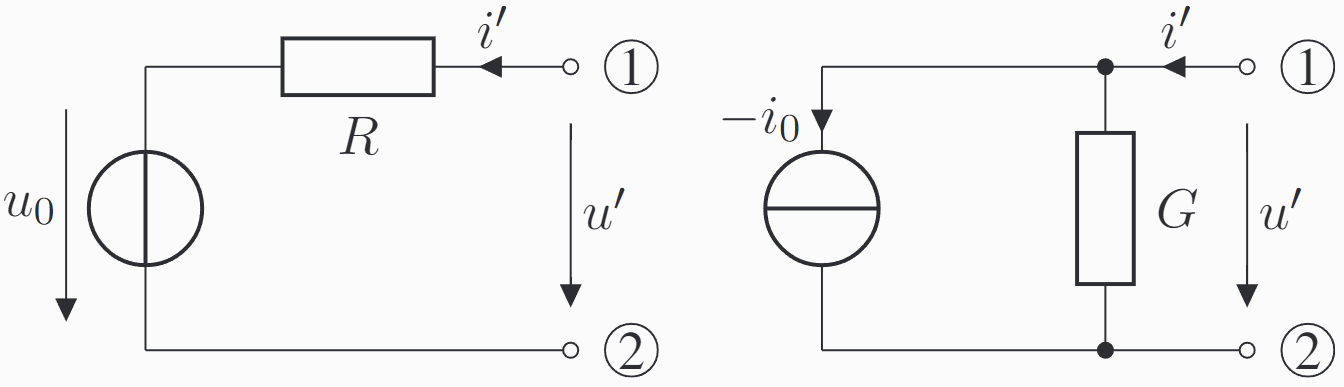
\includegraphics[width=6cm]{./img/source_conv.png}
        \end{center}
        \[i_0=\frac{u_0}R=u_0\cdot G\qquad u_0=\frac{i_0}{G}=i_0\cdot R \qquad R=\frac1G \qquad G= \frac 1R\]

        \textbf{Achtung}: Beachte die umgekehrte Richtung des Stromes $i_0$! $i_0$ fließt (in positiver Richtung normalerweise) am Knoten 1 heraus.
    }

    \sectionbox{
        \subsection{Linearisierung}
        Beispiel spannungsgesteuert, stromgesteuert analog\\
        $g_{\text{lin}} = \left. \frac{\partial i_{\mathcal F}}{\partial u_{\mathcal F}} \right|_{AP}$\\
        $\Delta i = i - I_{AP}$ \quad $\Delta u = u - U_{AP}$\\
        $\Delta i = g_{\text{lin}} \Delta u$\\
        $i_{\mathcal F,\text{lin}} = \Delta i + I_{AP} = \Delta u \cdot g_{\text{lin}} + U_{AP} = g_{\text{lin}}(u_{\mathcal F} - U_{AP}) + I_{AP}$
    }

    \sectionbox{
        \subsection{Ersatzschaltbilder}
        \begin{tabular}{ll}
            Konkaver Widerstand                                       & Konvexer Widerstand                                      \\
            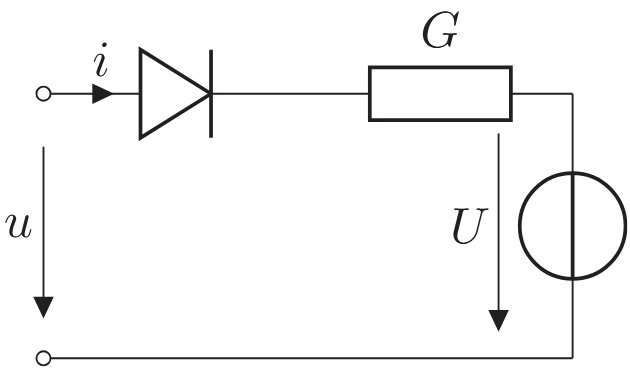
\includegraphics[scale = 0.2]{./img/konkave_resistor.png} & 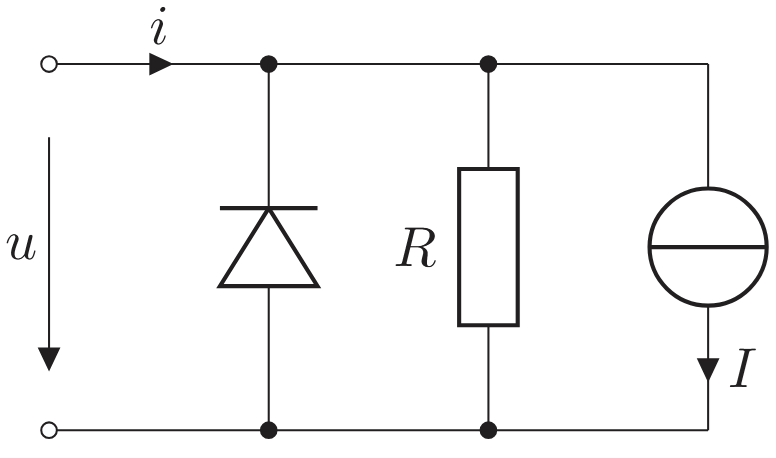
\includegraphics[scale = 0.2]{./img/konvex_resistor.png} \\
        \end{tabular}
    }

    \subsection{Liste}
    \begin{tabular}{@{}p{1.1cm}p{2.9cm}l}
        \parbox{1.3cm}{ Leerlauf                \\[5pt] 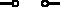
\includegraphics{./img/opencircuit.pdf} } & \parbox{2.5cm}{$u=\mathrm{beliebig}$ \\ $i=0$ \\ u, sl, v} & \parbox{1.8cm}{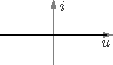
\includegraphics{./img/char/char_opencircuit.pdf} }  \\ \mrule
        \parbox{1.3cm}{ Kurzschluss             \\[5pt] 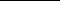
\includegraphics{./img/shortcircuit.pdf}  } & \parbox{2.5cm}{$u = 0$ \\ $i = \mathrm{beliebig}$ \\ u, sl, v} & \parbox{1.8cm}{ 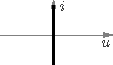
\includegraphics{./img/char/char_shortcircuit.pdf} } \\    \mrule
        \parbox{1.3cm}{ Nullator                \\[5pt] 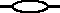
\includegraphics{./img/symb/symb_nullator.pdf} } & \parbox{2.5cm}{$u = 0 \quad i = 0$ \\ u, sl, v, dual zu sich selbst} & \parbox{1.8cm}{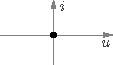
\includegraphics{./img/char/char_nullator.pdf} } \\ \mrule
        \parbox{1.3cm}{ Norator                 \\[5pt] 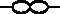
\includegraphics{./img/symb/symb_norator.pdf} } & \parbox{2.5cm}{$u = \mathrm{beliebig}$ \\ $i=\mathrm{beliebig}$ \\[0.5em] u, sl, a, dual zu sich selbst} & \parbox{1.8cm}{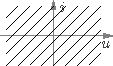
\includegraphics{./img/char/char_norator.pdf} } \\ \mrule
        \parbox{1.3cm}{ Widerstand              \\[5pt] 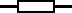
\includegraphics{./img/symb/symb_resistor.pdf} }& $\begin{array}{@{}cc} u = R \cdot i \\ i = G \cdot u \end{array} \quad G = \frac{1}{R}$ & \parbox{1.8cm}{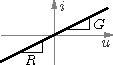
\includegraphics{./img/char/char_resistor.pdf} } \\ \mrule
        \parbox{1.3cm}{ \shortstack{Konkaver    \\Widerstand}   \\ 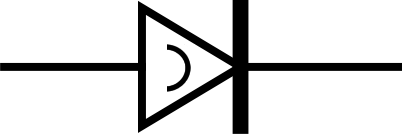
\includegraphics{./img/symb/symb_resistor_concave.png} }& $i=\begin{cases}0&\text{, }u\le U\\ G(u-U)&\text{, }u>U\end{cases}$ & \parbox{1.8cm}{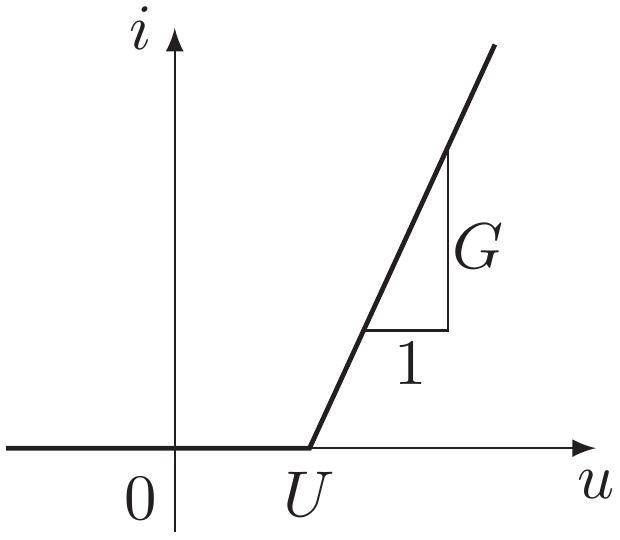
\includegraphics[width=1.8cm]{./img/char/char_resistor_concave.png} } \\ \mrule
        \parbox{1.3cm}{ \shortstack{Konvexer    \\Widerstand}   \\ 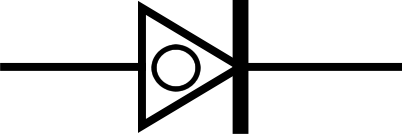
\includegraphics{./img/symb/symb_resistor_convex.png} }& \shortstack{ \shortstack{Dual zum\\\textbf{konkaven Widerstand}} \\ $u=\begin{cases}0&\text{, }i\le I\\ R(i-I)&\text{, }i>I\end{cases}$ }& \parbox{1.8cm}{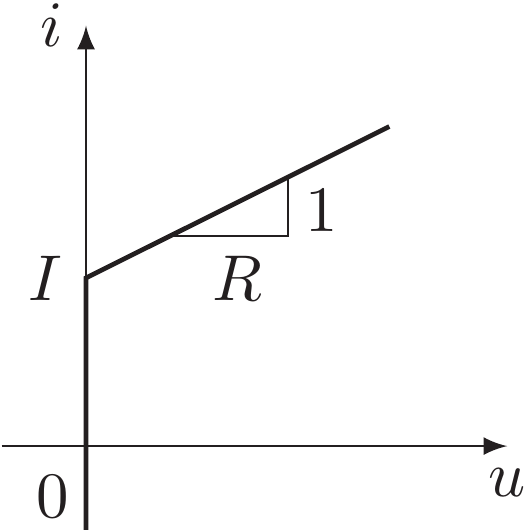
\includegraphics[width=1.6cm]{./img/char/char_resistor_convex.png} } \\ \mrule

        \parbox{1.3cm}{ Spannungsq.             \\[3pt] 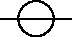
\includegraphics{./img/symb/symb_source_voltage.pdf} }& $\begin{array}{@{}ll} u = U_0 \\ i = \mathrm{beliebig}\end{array}$ & \parbox{1.8cm}{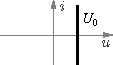
\includegraphics{./img/char/char_source_voltage.pdf} } \\ \mrule
        \parbox{1.3cm}{ Stromquelle             \\[3pt] 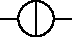
\includegraphics{./img/symb/symb_source_current.pdf} }& $\begin{array}{@{}ll} u = \mathrm{beliebig} \\ i = I_0 \end{array}$ & \parbox{1.8cm}{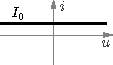
\includegraphics{./img/char/char_source_current.pdf} }    \\ \mrule
        \parbox{1.3cm}{ ideale Diode            \\[5pt] 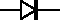
\includegraphics{./img/symb/symb_diode.pdf} }& $\begin{array}{@{}ll} u = 0 & \text{falls } i > 0 \\ i = 0 & \text{falls } u < 0\end{array}$ & \parbox{1.8cm}{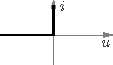
\includegraphics{./img/char/char_diode_ideal.pdf} } \\ \mrule
        \parbox{1.3cm}{ \shortstack{reale Diode \\pn Diode}  \\[5pt] 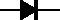
\includegraphics{./img/symb/symb_diode_real.pdf} }& $\begin{array}{@{}ll} u_D = u_T \cdot \ln \left(\frac{i_D}{I_S} + 1 \right) \\[0.7em] i_D = I_S \cdot \left( \exp \left(\frac{u_D}{U_T}\right) -1 \right) \end{array}$ & \parbox{1.8cm}{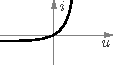
\includegraphics{./img/char/char_diode_real.pdf} } \\ \mrule
        \parbox{1.3cm}{ Photodiode              \\ 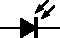
\includegraphics{./img/symb/symb_diode_photo.pdf} }& $i = I_{S} \left( e^{\frac{u_{D}}{U_{T}}} -1 \right) - i_L$ & \parbox{1.8cm}{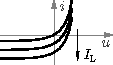
\includegraphics{./img/char/char_diode_photo.pdf} } \\ \mrule
        \parbox{1.3cm}{ Zenerdiode              \\ 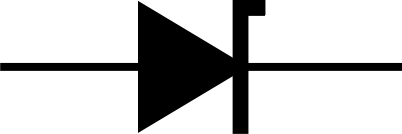
\includegraphics{./img/symb/symb_diode_zener3.png} }&\shortstack{ Durchbruch bei $u=U_Z$:\\ für $u\leq U_z$ stark leitend} & \parbox{1.8cm}{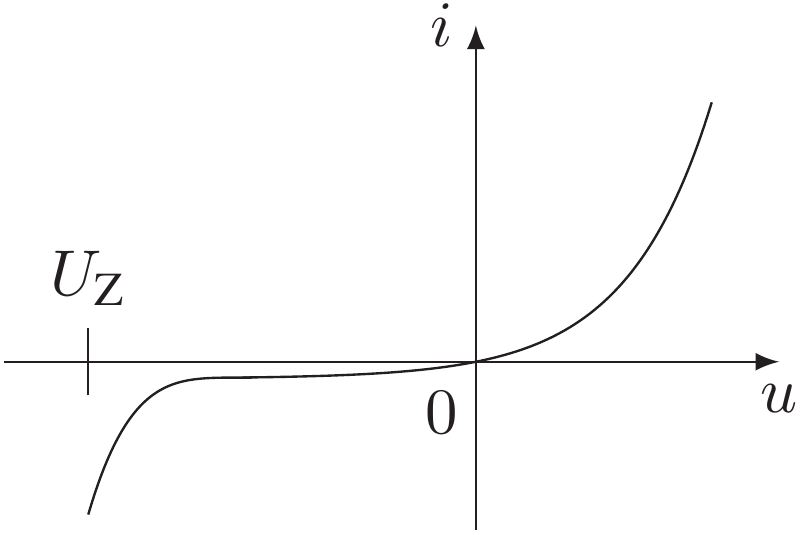
\includegraphics[width=1.8cm]{./img/char/char_diode_zener.png} } \\ \mrule
        \parbox{1.3cm}{ Tunneldiode             \\ 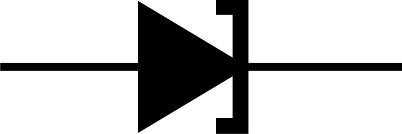
\includegraphics{./img/symb/symb_diode_tunnel2.png} }& \shortstack{Im gewissen Bereich wie ein\\\textbf{negativer Widerstand}} & \parbox{1.8cm}{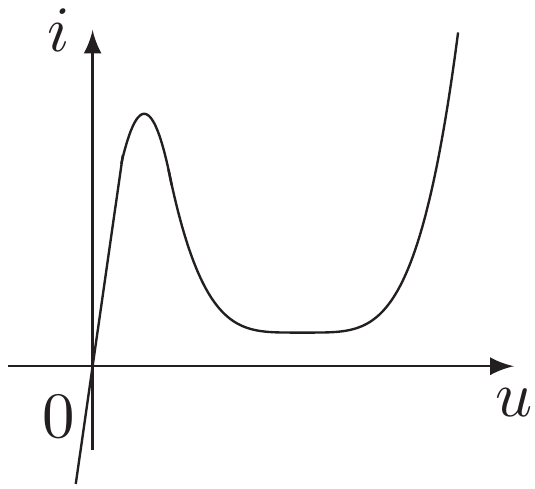
\includegraphics[width=1.7cm]{./img/char/char_diode_tunnel.png} }
    \end{tabular}

    \columnbreak
    % SECTION ====================================================================================
    \section{Resistive Zweitore}
    % ============================================================================================
    Ein Zweitor besteht aus zwei Eintoren.\\

    \subsection{Beschreibungsformen von Zweitoren}
    \begin{tabular}{@{}p{1.3cm}|ll@{}}
        Beschreibung                & nicht linear                                                                                                                          & linear                                 \\ \mrule
        \textbf{Implizit}           & $f_{\mathcal F}( \ul u, \underline i) = \ul 0$                                                                                        & $\mat{ \ma M & \ma N} \cdot \mat{\ul u \\ \ul i} = 0$ \\ \mrule
        \textbf{Parametrisch}       & $\begin{array}{@{}l} \ul u = u_{\mathcal F}(\ul \lambda) \\ \ul i=i_{\mathcal F}(\ul \lambda) \end{array}$ & $\mat{ \ul u                           \\ \ul i } = \mat{\utilde{ \bf U} \\ \utilde{ \bf I}} \cdot \ul c$  \vspace{2em} \\
        \textbf{Explizit}           & nicht linear                                                                                                                          & linear                                 \\\mrule
        Widerstand-beschreibung     & $\mat{ u_1                                                                                                                                                                     \\ u_2} = \mat{ r_1(i_1,i_2)\\ r_2(i_1,i_2) }$ & $= \mat{ U_0 \\ U_0} + \utilde{ \bf R} \mat{ i_1 \\ i_2} $ \\ \mrule
        Leitwert-beschreibung       & $\mat{ i_1                                                                                                                                                                     \\ i_2} = \mat{g_1(u_1,u_2) \\ g_2(u_1,u_2)}$ & $= \mat{ I_0 \\ I_0} + \utilde{ \bf G} \mat{ u_1 \\ u_2} $ \\ \mrule
        Hybrid-beschreibung         & $\mat{ u_1                                                                                                                                                                     \\ i_2} = \mat{h_1(i_1,u_2) \\ h_2(i_1,u_2)} $ & $= \ma{H} \cdot \mat{ i_1\\ u_2 }$\\ \mrule
        Inver. Hybrid- beschreibung & $\mat{ i_1                                                                                                                                                                     \\ u_2} = \mat{h'_1(u_1,i_2) \\ h'_2(u_1,i_2)}$ & $= \ma{H'} \cdot \mat{ u_1\\ i_2 }$ \\ \mrule
        Ketten-beschreibung         & $\mat{ u_1                                                                                                                                                                     \\ i_1} = \mat{a_1(u_2,-i_2) \\ a_2(u_2,-i_2)}$ & $= \ma{A} \cdot \mat{ u_2\\ -i_2 }$\\ \mrule
        Inver. Ketten- beschreibung & $\mat{ u_2                                                                                                                                                                     \\ i_2} = \mat{a'_1(u_1,-i_1) \\ a'_2(u_1,-i_1)}$ &  $= \ma{A'} \cdot \mat{ u_1\\ -i_1 }$
    \end{tabular}\\

    \subsection{Aufstellen der Zweitormatrix}
    \subsubsection{By Inspection}
    Gleichungen aufstellen und gesuchte Matrix daraus ableiten.
    \subsubsection{Kurzschluss-Leerlauf-Methode}
    Für jede steuernde Größe: (z.B. $\vec u = \ma R \vec i$)
    \begin{itemize}
        \item steuernde Größe festsetzen (zu Bsp. zuerst $i_1$ fest)
        \item restliche steuernde Größen auf 0 setzen (mit KS oder LL) (zu Bsp. $i_2=0A$)
        \item gesteuerte Größen in Abhängigkeit der Steuergrößen (die nicht 0 ist) ermitteln (zu Bsp. $u_1=R_a i_1, u_2=R_b i_1$)
        \item Für jede steuernde Größe wiederholen (zu Bsp. jetzt $i_2$ festsetzen, $i_1=0A$ setzen, $u_1, u_2$ in Abhängigkeit von $i_2$ ausdrücken)
    \end{itemize}
    \subsubsection{Quellenbehaftete lineare Zweitore}
    \begin{enumerate}\itemsep0pt
        \item Matrix des quellenfreien Zweitors bestimmen
        \item Quellvektor bestimmen (beide steuernden Größen auf null setzen)
        \item Schaltbild mit externen Quellen zeichnen je nach Beschreibungsform
    \end{enumerate}

    \sectionbox{
        \begin{tcolorbox}[colframe=red, colback=white]
            \textbf{Implizit $\ra$ Explizit}\\
            $\ma R = -\ma M^{-1}\ma N$\quad
            $\ma G = -\ma N^{-1}\ma M$\\
            \textbf{Explizit $\ra$ Implizit}\\
            $\ma 1 \vec u - \ma R \vec i = \vec 0$\quad
            $-\ma G \vec u + \ma 1 \vec i = \vec 0$\\
            \textbf{Parametrisch $\ra$ Explizit}\\
            $\ma R = \ma U \ma I^{-1}$\quad
            $\ma G = \ma I \ma U^{-1}$\\
            \textbf{Implizit $\ra$ Parametrisch}\\
            $\mat{\ma U\\\ma I} = \mat{-\ma M^{-1}\ma N\\\ma 1}$\quad
            $\mat{\ma U\\\ma I} = \mat{\ma 1\\-\ma N^{-1}\ma M}$\\
            \textbf{Parametrisch $\ra$ Implizit}\\
            $-\ma I \ma U^{-1} \vec u + \ma 1 \vec i = 0$\quad
            $\ma 1 \vec u - \ma U \ma I^{-1} \vec i = 0$
        \end{tcolorbox}
    }


    \subsection{Verschaltung von Zweitoren}
    % ============================================================================================================
    Es gibt sechs mögliche Verschaltungen.\\
    \begin{tabular}{@{}ll}
        Verschaltung & Bild                                                        \\ \hline
        \parbox{3cm}{Parallel: $g_{ges}=g_{\mathcal F1}+g_{\mathcal F2}$           \\ linear: $\ma G_{\ir ges} = \ma G_1 + \ma G_2$ \\ Umrechnung: } & \parbox{2.5cm}{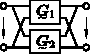
\includegraphics{./img/ztv_leitwert.pdf}}\\[2em]
        \parbox{3cm}{Serie: $r_{ges}=r_{\mathcal F1}+r_{\mathcal F2}$              \\ linear: $\ma R_{\ir ges} = \ma R_1 + \ma R_2$} & \parbox{2.5cm}{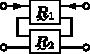
\includegraphics{./img/ztv_widerstand.pdf}}\\[2em]
        \parbox{3cm}{Hybrid: $h_{ges}=h_{\mathcal F1}+h_{\mathcal F2}$             \\ linear: $\ma H_{\ir ges} = \ma H_1 + \ma H_2$ \\ auch genannt: Serien-Parallel} & \parbox{2.5cm}{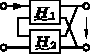
\includegraphics{./img/ztv_hybrid.pdf}}\\[2em]
        \parbox{3.5cm}{Hybrid Inv.: $h'_{ges}=h_{\mathcal F1}+h'_{\mathcal F2}$    \\ linear: $\ma H'_{\ir ges} = \ma H'_1 + \ma H'_2$ \\ auch genannt: Parellel-Serie} & \parbox{2.5cm}{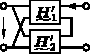
\includegraphics{./img/ztv_hybrid_inv.pdf}}\\[2em]
        \parbox{3cm}{Kette: $a_{ges}=a_{\mathcal F1} \cdot a_{\mathcal F2}$        \\ linear: $\ma A_{\ir ges} = \ma A_1 \cdot \ma A_2$} & \parbox{2.5cm}{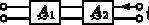
\includegraphics{./img/ztv_kette.pdf}}\\[2em]
        \parbox{3cm}{Kette Inv: $a'_{ges}=a'_{\mathcal F2} \cdot a'_{\mathcal F1}$ \\ linear: $\ma A'_{\ir ges} = \ma A'_2 \cdot \ma A'_1$} & \parbox{2.5cm}{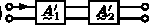
\includegraphics{./img/ztv_kette_inv.pdf}}\\
    \end{tabular}

    \subsection{Liste von Zweitoren}
    \subsubsection{VCCS}
    $\ma A = \mat{0&-\frac{1}{g}\\0&0}$\quad
    $\ma G = \mat{0&0\\g&0}$
    \subsubsection{CCCS}
    $\ma A = \mat{0&0\\0&-\frac{1}{\beta}}$\quad
    $\ma H = \mat{0&0\\\beta&0}$
    \subsubsection{VCVS}
    $\ma A = \mat{\frac{1}{\mu}&0\\0&0}$\quad
    $\ma H' = \mat{0&0\\\mu&0}$
    \subsubsection{CCVS}
    $\ma A = \mat{0&0\\\frac{1}{r}&0}$\quad
    $\ma R = \mat{0&0\\r&0}$

    \subsubsection{Nullor}
    $\ma A = \mat{0&0\\0&0}$\quad
    $\ma M = \mat{1&0\\0&0}$\quad
    $\ma N = \mat{0&0\\1&0}$\\
    Eigenschaften: Quellenfrei, streng linear

    \subsubsection{Übertrager (z.B. Transformator)}
    $\ma A = \mat{\text{ü}&0\\0&\frac{1}{\text{ü}}}$\quad
    $\ma H = \mat{0&\text{ü}\\\text{-ü}&0}$\quad
    $\ma H' = \mat{0&-\frac{1}{\text{ü}}\\\frac{1}{\text{ü}}&0}$\quad\\
    $\ma M = \mat{1&\text{-ü}\\0&0}$\quad
    $\ma N = \mat{0&0\\\text{ü}&1}$\quad

    $R_{in}=\frac{u_1}{i_1}=\text{ü}^2 R_L$\\
    Eigenschaften: verlustlos(ideal)


    \subsubsection{Gyrator}
    Schaltet man an Tor 2 (bzw. an dem Tor, auf das $R_d$-Pfeil zeigt) ein Element an, so beobachtet man an Tor 1 das duale Element.\\
    Schaltet man an Tor 1 ein Element an, so beobachtet man an Tor 2 das duale, \textbf{umgepolte} Element.\\
    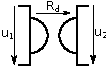
\includegraphics[scale=.8]{./img/symb/symb_gyrator.pdf}
    $\begin{array}{l}
            \ma A=\mat{0 & R_d \\ \frac{1}{R_d} & 0}\mathrm{\quad}\ma R = \mat{0&-R_d\\R_d&0}\\ \mathrm{\quad} G = \mat{0&G_d\\-G_d&0}\mathrm{\quad}\mathcal F_{in}=\mathcal F^d
        \end{array}$\\
    Eigenschaften: streng linear, verlustlos für $R_1=R_2$\\

    \subsubsection{Negativ-Immitanz-Konverter}
    $\ma A = \mat{-k&0\\0&\frac{1}{k}}$\quad
    $\ma H = \mat{0&-k\\-k&0}$\\
    $R_{in}=\frac{u_1}{i_1}=-k^2R$ \quad $-k^2 R:$\ negativer Widerstand\\
    Eigenschaften: streng linear, aktiv\\
    Nullator überhalb $R$ (Nullor-Realisierung): $k=-1$\\
    Norator überhalb $R$ (Nullor-Realisierung): $k=+1$

    \sectionbox{
        \subsection{NIK allgemein (Polung beachten)}
        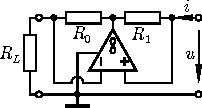
\includegraphics[scale = 0.85]{./img/NIK.pdf} \qquad 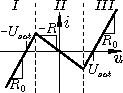
\includegraphics{./img/char/char_NIK.pdf}\\
        \begin{tabular}{cll}
            I   & negative Sättigung $u_d < 0 \Leftrightarrow u_{out}=-U_{sat}$                                  \\
                & $u = R_0 i - U_{sat}$                                                                          \\ % < \frac{R_L}{R_L + R_1} \cdot U_{sat}$\\
            II  & linearer Bereich $u_d = 0$                                                                     \\
                & $u = - \frac{R_0}{R_1} R_L \cdot i$ \qquad \quad $-U_{sat} < \frac{R_L + R_1}{R_L}u < U_{sat}$ \\
            III & positive Sättigung $u_d > 0 \Leftrightarrow u_{out}=U_{sat}$                                   \\
                & $u = R_0 i + U_{sat}$                                                                          % < \frac{R_L}{R_L + R_1} \cdot U_{sat}$\\
        \end{tabular}
    }

    \subsection{Dualwandlung}
    $\mat{\ma U\\\ma I}^d = \mat{R_d\ma I\\\frac{1}{R_d}\ma U}$\\
    $\ma G^d = \frac{1}{R_d^2} \ma R$ \quad $\ma R^d = R_d^2 \ma G$

    \subsection{Linearisierung}
    \begin{tabular}{ll}
        Großsignal                 & Kleinsignal                  \\
        $i=I_{\ir AP}+\Delta i$ \  & \ $\Delta i= i - I_{\ir AP}$ \\
        $u=U_{\ir AP}+\Delta u$ \  & \ $\Delta u= u - U_{\ir AP}$ \\
    \end{tabular}
    \\
    $\vec i = \vec g(\vec u)$\quad$\Delta \vec i \approx \ma G \cdot \Delta \vec u$\\
    $\ma G$ ist die Jakobimatrix $\left. \frac{\partial g_i(\vec u)}{\partial u_j} \right|_{U_{\ir AP}} = \left. \mat{
            \frac{\partial g_1}{\partial u_1} & \frac{\partial g_1}{\partial u_2}\\
            \frac{\partial g_2}{\partial u_1} & \frac{\partial g_2}{\partial u_2}
        }\right|_{U_{AP}}$\\
    $\Delta \vec u \approx \ma R \cdot \Delta \vec u$\\
    Großsignal: $i \approx I_{\ir AP} + G(U_{\ir AP}) \cdot (u - U_{\ir AP})$\\[1em]

    Implizite Linearisierung: $\Delta \vec f(\Delta \vec u, \Delta \vec i) = \ma M \Delta \vec u + \ma N \Delta \vec i$\\
    $\ma M := \mat{ \frac{\partial f_1}{\partial u_1} & \frac{\partial f_1}{\partial u_2} \\[0.5em] \frac{\partial f_2}{\partial u_1} & \frac{\partial f_2}{\partial u_2} }$ \quad
    $\ma N := \mat{ \frac{\partial f_1}{\partial i_1} & \frac{\partial f_1}{\partial i_2} \\[0.5em] \frac{\partial f_2}{\partial i_1} & \frac{\partial f_2}{\partial i_2} }$

    % SECTION ====================================================================================
    \section{Eigenschaften von Ein- und Mehrtoren}
    % ============================================================================================
    Ein Mehrtor $\mathcal F(\vec u, \vec i)$ ist ...

    \textbf{Resistiv}: Gedächtnislos; nur von $u$ und $i$ abhängig\\
    \textbf{Zeitvariant}: Betriebsraum kann sich ändern\\
    \textbf{Reziprozität}: $\ma G^T$ = $\ma G$, $\ma R^T$ = $\ma R$, $\det (\ma A)$ = 1, $\det (\ma {A'})$ = 1, $h_{21} = -h_{12}$, $h'_{21} = -h'_{12}$, $\ma U^T\ma I$ = $\ma I^T\ma U$\\
    \textbf{Symmetrie}: $r_{11} = r_{22}$ und $r_{12}=r_{21}$, \\
    $\ma R = \ma P\ma R\ma P$, $\ma G = \ma P \ma G \ma P$ mit $\ma P = \mat{0 & 1 \\ 1 & 0}$, \\
    $\ma A = \ma A'$ \! \! \! \! $\det \ma H = \det \ma H' = 1$

    \tablebox{
        \begin{tabular*}{\columnwidth}{@{\extracolsep\fill}ll@{}}
            \ctrule
            Eigenschaft & Bedingung\\ \mrule
            $\mathcal F$ quellenfrei & $\vec 0 \in \mathcal F$; enthält den Ursprung \\
            $\mathcal F$ streng linear & $(ku, ki) \in F$ \quad $ (u_1 + u_2, i_1 + i_2) \in F$ \\
            \cbrule
            Nur für Eintore:\\
            ungepolt & Kennlinie punktsymm. zum Ursprung \\
            & $\mathcal F(u,i)=\mathcal F(-u,-i)$
        \end{tabular*}
    }

    \subsection{Linearität}
    Linear: $(ku, ki) \in F$ \quad $(u_1 + u_2, i_1 + i_2) \in F$ (Kennlinie gerade) \\
    Streng Linear: linear + quellenfrei, (Gerade durch Ursprung)\\

    \subsection{Zeitvarianz}
    Ein Mehrtor heißt zeitvariant, wenn sich sein Betriebsraum mit der Zeit ändern kann, ansonsten
    ist es Zeitinvariant.

    \subsection{Steuerung}
    Ein Bauelement ist von einer Größe gesteuert, wenn die jeweilige explizite Beschreibung existiert.\\
    \begin{tabular*}{\columnwidth}{@{\extracolsep\fill}llll@{}}
        Stromgesteuert: & $u=\mathcal R(i)$ & Spannungsgestuert: & $i=\mathcal G(i)$\\
        Ladungsgesteuert: & $u=\mathcal C^{-1}(q)$ & Flussgesteuert: & $i=\mathcal L^{-1}(\Phi)$
    \end{tabular*}

    \subsection{Leistungsbetrachtung}
    Verlustlosigkeit: $\ma U^T\ma I + \ma I^T \ma U = 0$ oder $\ma R$ schiefsymm.\\
    Leistung: $P(t)=\ul u^T \cdot \ul i=u_1 i_1 + \dotsc + u_n i_n$ \\
    \begin{tabular*}{\columnwidth}{@{\extracolsep\fill}lll@{}}
        Passiv: & $\forall \mathcal F(u,i): P(t)\ge 0$ & Kennlinie nur I. oder III. Quadrant\\
        Aktiv: & $\exists \mathcal F(u,i): P(t)<0$ & Kennlinie im II. oder IV. Quadrant\\
        Verlustlos: & $\forall \mathcal F(u,i): P(t)=0$ & Kennlinie nur auf Koordinatenachsen\\
    \end{tabular*}\\
    Merke: Alle Mehrtore die nur aus passiven Bauelementen(R,C,L,...) bestehen, sind selbst passiv!
    inkremental passiv:\\
    letztendlich passiv: $\exists U,I>0 \ \forall (u,i) \in \mathcal F : (|u| > U \lor |i| > I \ \Rightarrow \ ui > 0)$\\
    Alle realen Bauteile sind letztendlich passiv, da sonst unendlich viel Energie entstehen würde.\\

    % SECTION ====================================================================================
    \section{Operationsverstärker (OpAmp)}
    % ============================================================================================
    Der Operationsverstärker ist ein elektronischer Verstärker.

    \sectionbox{
        \subsection{Idealer Operationsverstärker}

        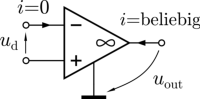
\includegraphics{./img/opamp.pdf} \qquad 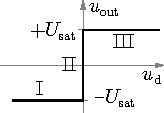
\includegraphics{./img/char/char_opamp.pdf}\\[2em]
        \begin{tabular}{lll}
            \parbox{3cm}{\textbf{\large ESB I}   \\ negativer Sättigungsbereich \\ $u_{\ir d} < 0$  \\ $u_{\ir out} = - U_{\ir sat}$} & \parbox{3cm}{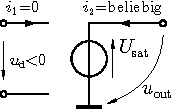
\includegraphics[scale = 0.9]{./img/opamp_esb_1.pdf} }\\[4em]
            \parbox{3cm}{\large \textbf{ESB II}  \\ streng linearer Bereich \\ $u_{\ir d} = 0$ \\ $\abs{ u_{\ir out} } \le U_{\ir sat}$} & \parbox{3cm}{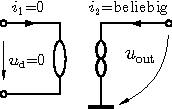
\includegraphics[scale = 0.9]{./img/opamp_esb_2.pdf} }\\[4em]
            \parbox{3cm}{\textbf{\large ESB III} \\ positiver Sättigungsbereich \\ $u_{\ir d} > 0$  \\ $u_{\ir out} = + U_{\ir sat}$} & \parbox{3cm}{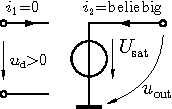
\includegraphics[scale = 0.9]{./img/opamp_esb_3.pdf} }
        \end{tabular}
    }

    \sectionbox{
        Differenzverstärkung $\nu_d$: $\nu_d=\frac{u_{out}}{u_{in}}$
    }


    \begin{tabular}{ll}
        Invertierender Verstärker                                & Nichtinvert. Verstärker                                              \\
        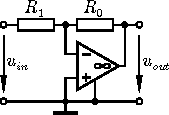
\includegraphics[scale = 0.9]{./img/invamp.pdf}          & 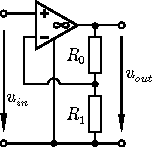
\includegraphics[scale = 0.9]{./img/notinvamp.pdf}                   \\
        $u_{\ir out} = \frac{-R_0}{R_1} u_{in}$                  & $u_{\ir out} = \left( 1+ \frac{R_0}{R_1} \right) u_{in}$             \\[0.5em] \mrule
        Differenzierer                                           & Integrierer                                                          \\
        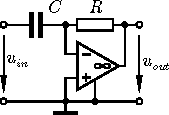
\includegraphics[scale = 0.9]{./img/differenzierer.pdf}  & 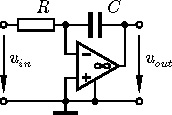
\includegraphics[scale = 0.9]{./img/integrierer.pdf}                 \\
        $u_{\ir out} = -RC \cdot \dot u_{in}$                    & $u_{\ir out} = -\frac{1}{RC} \int\limits^{t_1}_{t_0} u_{in} \diff t$ \\ \mrule
        Logarithmierer                                           & Exponenzierer                                                        \\
        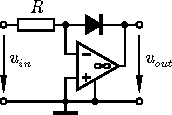
\includegraphics[scale = 0.9]{./img/logarithmierer.pdf}  & 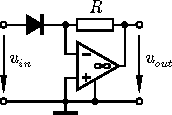
\includegraphics[scale = 0.9]{./img/exponenzierer.pdf}               \\
        $u_{\ir out} = -U_T \ln \frac{u_{in}}{R \cdot I_S}$      & $u_{\ir out} = -R \cdot I_S \exp \left( \frac{u_{in}}{U_T} \right)$  \\ \mrule
        Spannungsfolger                                          & Addierer                                                             \\
        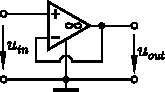
\includegraphics[scale = 0.9]{./img/voltagefollower.pdf} & 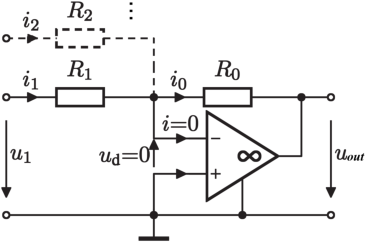
\includegraphics[scale = 0.45]{./img/addierer.pdf}                   \\
        $u_{\ir out} = u_{in}$ \quad $i_{in} = 0$                & $u_{\ir out} = -R_0 \sum \frac{u_i}{R_i}$                            \\ \mrule
        NIK                                                      & Potenzialdifferenzverstärker                                         \\
        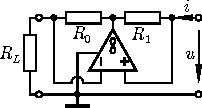
\includegraphics[scale = 0.8]{./img/NIK.pdf}             & 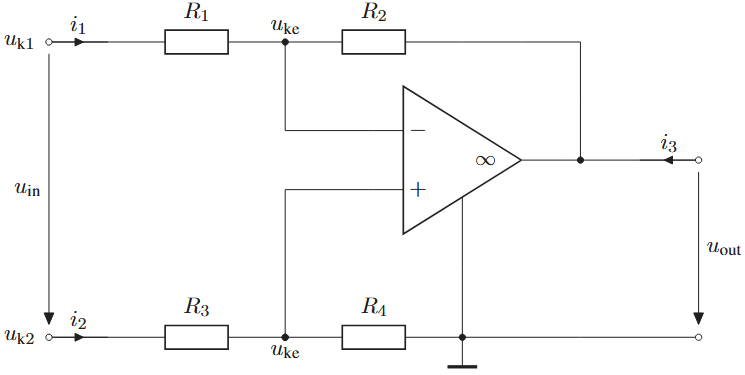
\includegraphics[scale = 0.2]{./img/potdiffamp.png}                  \\
        $u = -R_L \cdot i$                                       & $\nu_d=-\frac{R_2}{R_1}=-\frac{R_4}{R_3}$                            \\
    \end{tabular}


    \section{Resistive Mehrtore}
    \subsection{Beschreibungsformen}
    Analog zu Zweitoren, nur mit mehr Dimensionen und es gibt sehr viele, nicht mehr benannte Hybridbeschreibungen.
    \subsubsection{Dimensionen eines p-Tores}
    Betriebsraum: p\\
    Menge an lin. unabh. Gleichungen zur Beschreibung: p\\
    $\ma R\in \mathbb R^{p \times p}$ mit Torvektor $\in \mathbb R^{p \times 1}$
    \subsection{Spezielle Mehrtore}
    \subsubsection{Mehrtorübertrager}
    $\ma H_{\text{Übertrager}} = \mat{\ma 0 & \ma H_{a,b}\\-\ma H^T_{a,b}&\ma 0}$\\
    $\ma H'_{\text{Übertrager}} = \mat{
            0 & -\frac{1}{"u_2} & -\frac{1}{"u_3} & \cdots & -\frac{1}{"u_p}\\
            \frac{1}{"u_2} & 0 & 0 & \cdots & 0\\
            \frac{1}{"u_3} & 0 & 0 & \cdots & 0\\
            \vdots & \vdots & \vdots & \ddots & \vdots\\
            \frac{1}{"u_p} & 0 & 0 & \cdots & 0}$\\
    Eigenschaften: Verlustlos und Reziprok

    \subsubsection{Zirkulator}
    $\ma M = \ma 1$ \quad $\ma N = \mat{
            0 & -R & +R\\
            +R &  0 & -R\\
            -R & +R &  0}$\\
    $\ma R = -\ma M^{-1}\ma N = -\ma N = \mat{
            0 & +R & -R\\
            -R &  0 & +R\\
            +R & -R &  0} = -\ma R^T$\\
    Eigenschaften: Verlustlos, Nicht reziprok, Schiefsymmetrisch\\
    $p_1 = u_1i_1 = \frac{u_0^2}{4R} \geq 0W$\\
    $p_2 = u_2i_2 = -\frac{u_0^2}{4R} = -p_1 \leq 0W$\\
    $P_3 = u_3i_3 = 0W$\\
    Die an einem Tor aufgenommene Leistung wird in Pfeilrichtung an das nächste weitergegeben.

    \subsubsection{Multiplizierer}
    $\mat{i_1\\i_2\\u_3} = h\left(\mat{u_1\\u_2\\i_3}\right) = \mat{0\\0\\\frac{u_1u_2}{U_M}}$\quad$u_3=\frac{u_1u_2}{U_M}$, $U_M$ Multipliziererkonstante

    \subsubsection{Dividierer}
    $\mat{i_1\\i_2\\u_3} = h\left(\mat{u_1\\u_2\\i_3}\right) = \mat{0\\0\\\frac{u_1}{u_2}U_D}$\quad$u_3=\frac{u_1}{u_2}U_D$, $U_D$ Dividiererkonstante, $U_D = -U_M$\\
    Realisierung z.B. mit Multiplizierer in Rückkopplungspfad von OpAmp.

    % SECTION ====================================================================================
    \section{Allgemeine Analyseverfahren}
    % ============================================================================================

    \sectionbox{

        \subsection{Kirchhoff-Gesetze}
        Konzentriertheitshypothese: $d \ll \lambda$ mit \\
        $d = $ Größe der Schaltung, Wellenlänge $\lambda = c T$ \\

        %Knotenregel \emph{KCL}: $ \sum \limits_{\text{Knoten}}i_{\ir j} (t) = 0$ (heraußfließende Ströme positiv) \\
        %Maschenregel \emph{KVL}: $ \sum \limits_{\text{Umlauf}} u_{\ir j} (t) = 0$ (Spannungen in Umlaufrichtung positiv)

        \tablebox{
            \begin{tabular*}{\columnwidth}{@{\extracolsep\fill}ll@{}} \trule
                $\underset{\text{Kirchoff's Current Law}}{\text{\large Stromgesetz \textbf{KCL}}}$ & $\underset{\text{Kirchoff's Voltage Law}}{\text{\large Spannungsgesetz \textbf{KVL}}}$ \\ \mrule
                Knotenregel & Maschenregel\\[0.5em]
                $\displaystyle \sum\limits_{\ir Knoten} i_k (t) = 0 $ & $\displaystyle \sum\limits_{\ir Masche} u_m (t) = 0 $ \\[1.5em]
                rausfließende Ströme positiv & Spannungen in Umlaufrichtung positiv \\
                Maxwell: $\mathrm{div}\, \vec j = 0$ & Maxwell: $\mathrm{rot}\, \vec E = 0$ \\
                $(n-1)$ Gleichungen & $b-(n-1)$ Gleichungen\\ \brule
            \end{tabular*}
        }

    }

    \sectionbox{
        \subsection{Baumkonzept}
        $b$: Menge an Zweigen (Baumkanten + Verbindungskanten)\\
        $n$: Anzahl an Knoten\\
        \textbf{Baum}: Teilgraph des Netzwerkgraphen, der
        \begin{itemize}
            \item alle Knoten enthält und Verbindungen zwischen allen Knoten (man kommt von eimen Knoten zu jedem anderen)
            \item $n-1$ Baumkanten hat, die die Verbindungen zwischen den Knoten herstellen
            \item keine validen KVL-Umläufe hat (man darf nur mit Baumkanten kein KVL aufstellen können)
        \end{itemize}
        \textbf{Nummerierung}: erst Baumkanten nummerieren, dann Verbindungskanten.\\
        \textbf{KVL}: Pro Verbindungskante eine Masche, die sonst nur Baumkanten enthält:    $\mat{\ma B_b& \ma 1_s}\mat{\vec u_b\\ \vec u_v} = \vec{0}$
        \hfill($s=b-(n-1)$ Gleichungen)\\
        \textbf{KCL}: Bilden von (Super-)Knoten so, dass nur eine Baumkante durch den Knoten geht und ansonsten nur Verbindungskanten, Vorzeichen der Baumkante ist positiv: $\mat{\ma 1_{n-1}&\ma A_v}\mat{\vec i_b\\ \vec i_v} = \vec 0$
        \hfill($n-1$ Gleichungen)\\
        $\vec u_b$: Vektor an Spannungen, die zu den Baumkanten gehören \\
        $\vec u_v$: Vektor an Spannungen, die zu den Verbindungskanten gehören\\
        $\ma A_v = -\ma B_b^T$ gilt (NUR!) beim Baumkonzept!\\

        \resizebox{\columnwidth}{!} {
            \begin{tabular}{l|l|l}
                    & Nullraum                         & Bildraum               \\ \hline
                KCL & $\ma A \vec i = \mat{\ma 1_{n-1} & \ma A_v} \mat{\vec i_b \\ \vec i_v}=\vec 0$ & $\vec i = \ma B^T \vec i_v=\mat{\ma B_t^T \\ \ma 1_s}\vec i_v$ \\ \hline
                KVL & $\ma B \vec u = \mat{\ma B_b     & \ma 1_s}\mat{\vec u_b  \\ \vec u_v} = \vec 0$ & $\vec u = \ma A^T \vec u_b = \mat{\ma 1_{n-1} \\ \ma A_v} \vec u_b$
            \end{tabular}
        }

        % \textbf{KVL-/KCL-Darstellungen}\\
        % KVL (Nullraumdarst.): $\ma B \vec u = \vec 0$\\
        % KCL (Bildraumdarst.): $\vec i = \ma B^T \vec i_v$
    }

    \sectionbox{
        \subsection{Knoteninzidenzmatrix}
        Knoteninzidenzmatrix: $\ma A = \mat{\alpha_{11} &  \ldots & \alpha_{1b} \\ \vdots & &  \\ \alpha_{n-1,1} & \ldots & \alpha_{n-1,b}}$\\
        \textbf{Aufstellen}
        \begin{itemize}\itemsep0pt
            \item Wählen des Bezugsknotens
            \item Für alle Knoten außer Bezugsknoten:
            \item[-] Strom fließt aus dem Knoten heraus $\Rightarrow \alpha = +1$
            \item[-] Strom fließt in den Knoten hinein $\Rightarrow \alpha = -1$
        \end{itemize}
        \textbf{KVL-/KCL-Darstellungen}\\
        KCL (Nullraumdarstellung): $\ma A \vec i = \vec 0$\\
        KVL (Bildraumdarstellung): $\vec u = \ma A^T\vec u_k$ ($\vec u_k$ ist Vektor der Knotenpotenziale)
    }

    \sectionbox{
        \subsection{Spannungsinzidenzmatrix}
        Spannungsinzidenzmatrix: $\ma B = \mat {\alpha_{11} & \ldots & \alpha_{1,b} \\ \vdots & &  \\ \alpha_{s,1} & \ldots & \alpha_{s,b}}$\\
        \textbf{Aufstellen}\\
        Elementare Maschen (Maschen, die keine Kanten schneiden) in Nullraumdarst. aufstellen (Richtung frei wählbar)\\
        \textbf{KVL-/KCL-Darstellungen}\\
        KVL (Nullraumdarst.): $\ma B \vec u = \vec 0$\\
        KCL (Bildraumdarst.): $\ma B^T \vec i_m = \vec i$
    }

    \subsection{Tellegenscher Satz}
    $u^Ti = 0$
    \begin{itemize}
        \item Der Spannungsvektor steht immer senkrecht zum Stromvektor ($\ma A\ma B^T = \vec 0$ bzw. $\ma B\ma A^T = \vec 0$).
        \item Hat man entweder die $\ma A$ oder $\ma B$ Matrix gefunden, so kann man die andere ausrechnen, da das Innenprodukt einer KVL-Gleichung und einer KCL-Gleichung gleich $0$ ist. Jede Zeile von $A$ mal jede Zeile von $B$ gleich $0$
        \item Gilt für zwei verschiedene Schaltungen 1 und 2: $\vec u^{(1), T} \vec i^{(2)}=0$, so ist deren Struktur identisch.
    \end{itemize}

    \subsection{Die Tableau-Gleichung}
    ... beschreibt ein Netzwerk vollständig bezüglich Verschaltung und Bauteilverhalten. Oberen zwei Zeilen der Matrix liefern die $b$ KVL-/KCL-Gleichungen. Der untere Teil liefert die $b$ Elementgleichungen.\\
    $\begin{matrix}(b-(n-1)) \\ (n-1) \\ (b)\end{matrix} \mat{\ma B&\ma 0\\\ma 0&\ma A\\\ma M & \ma N}\mat{\vec u\\\vec i} = \mat{\vec 0\\\vec 0\\\vec e}$\\
    $\ma T^{2b \times 2b} = \mat{ \ma B & \ma 0 \\ \ma 0 & \ma A \\ \ma M & \ma N}$\\
    ($e = 0 \Leftrightarrow$ keine Quellen enthalten)

    \subsection{Newton-Raphson-Algorithmus}
    Nullstellensuche impliziter Beschreibungen $f(\vec u, \vec i)=f(\vec x^{(k)})$ mit $\vec x^{(k)}=\mat{\vec u \\ \vec i}$
    \begin{enumerate}
        \item Jacobimatrix $\ma J(\vec x^{(k)})$ aus den nichtlinearen impliziten Gleichungen finden. Eine Zeile pro nichtlinearem Element, Spalten abgeleitet nach $\delta u_1, \delta u_2, \delta i_1, \delta i_2$ usw.
        \item Tangente des 0. Linearisierungspunktes (gegebene Initialisierung $\vec x^{(0)}$) bestimmen und gleich 0 setzen: \\
              $t^{(0)}=f(\vec x^{(0)})+\ma J(\vec x^{(0)})(\vec x^{(1)}-\vec x^{(0)})=0$
        \item Gefundene Gleichung für $\vec x^{(1)}$ in Tableau-Gleichungssystem einsetzen und nach $\vec x^{(1)}$ auflösen, um den nächsten (Initialisierungs-)Punkt zu finden. Mit den neuen Punkt zu Schritt 2 gehen (bzw. alle Größen der Schaltung bestimmen, um nächsten Linearisierungspunkt zu erhalten).
        \item Fehler $\epsilon_1=f(x^{(1)})$
    \end{enumerate}

    \subsection{Maschenstromanalyse}
    $\mat{\ma B & \ma 0 & \ma 0 \\ \ma 0 & \ma 1 & \ma{-B}^T \\ \ma M & \ma N & \ma 0}=\mat{\vec u \\ \vec i \\ \vec i_m}=\mat{\vec 0 \\ \vec 0 \\ \vec e} \begin{matrix} \\ (3b-(n-1)) \\ \end{matrix}$\\
    Voraussetzung: Alle Elemente stromgesteuert\\
    Wird ein Strom in einem Zweig nur von einer Masche berührt, so ist er gleich dem Maschenstrom, wird ein Strom in einem Zweig von mehreren Maschen berührt, so ist er gleich der Summe der einzelnen Maschenströme

    \subsection{Knotenspannungsanalyse}
    $\mat{\ma{-A}^T & \ma 1 & \ma 0 \\ \ma 0 & \ma 0 & \ma A \\ 0 & \ma M & \ma N}=\mat{\vec u_k \\ \vec u \\ \vec i}=\mat{\vec 0 \\ \vec 0 \\ \vec e} \begin{matrix}(b) \\ (n-1) \\ (b)\end{matrix}$

    \subsubsection{reduzierte Knotenspannungsanalyse}
    \boxed{ \underset{\text{Knotenleitwertsmatrix}}{\ma Y_{\ir k}} \cdot \underset{\text{Spannungsvektor}}{\vec u_{\ir k}} = \underset{\text{Stromquellenvektor}}{\vec i_{\ir q}} } $(n-1 \times n-1)$\\
    $- \ma A \ma N^{-1} \ma M \ma A^T \vec u_k=-\ma A \ma N^{-1} \vec e$\\
    Vorgehen:
    \begin{enumerate}\itemsep0pt
        \item Nicht lineare Elemente linearisieren
        \item Nicht spannungsgesteuerte Elemente (dual)wandeln
        \item Aufstellen der Leitwertsmatrix $\ma Y'_k$
        \item Bestimmung des Stromquellenvektors $\vec i'_q$
        \item Einbau des Nullators: Addition der Spalten von $\ma Y'_k$ an denen er anliegt \& eine Spalte streichen. Z.B. Nullator zwischen \textcircled{1} und \textcircled{2}: Addiere Spalte von $u_{k1}$ auf Spalte von $u_{k2}$ und streiche Spalte $u_{k2}$ sowie $u_{k2}$ in $\vec u_k'$.
        \item Einbau des Norators: Addition der Zeilen \& eine Zeile streichen: Z.B. Norator zwischen \textcircled{1} und \textcircled{2}: Addiere Zeile von \textcircled{2} auf Zeile von \textcircled{1} und streiche Zeile \textcircled{2} sowie die \textcircled{2}. Zeile von $\vec i_q'$

    \end{enumerate}
    Spezialfall: Nullator/Norator mit Masse verbunden: Spalte/Zeile der Spannung/des Knotens streichen, der mit dem Nullator/Norator verbunden ist
    \subsubsection{Aufstellen der Knotenleitwertsmatrix}
    \tiny
    \begin{tabular}{ll}
        $\ma {Y_k} = \kbordermatrix{ & u_{k\alpha} &                                   & u_{k\beta}                                                                                     &                                  & u_{k\gamma}                                                                                  \\
        \alpha                       &             &                                   &                                                                                                & \ldots                           & G_d                                                                                          \\
                                     &             &                                   &                                                                                                &                                  & \vdots                                                                                       \\
        \beta                        &             &                                   &                                                                                                & \ldots                           & -G_d                                                                                         \\
                                     & \vdots      &                                   & \vdots                                                                                         &                                  & \vdots                                                                                       \\
        \gamma                       & -G_d        & \ldots                            & G_d                                                                                            & \ldots\\}$ & \parbox{3cm}{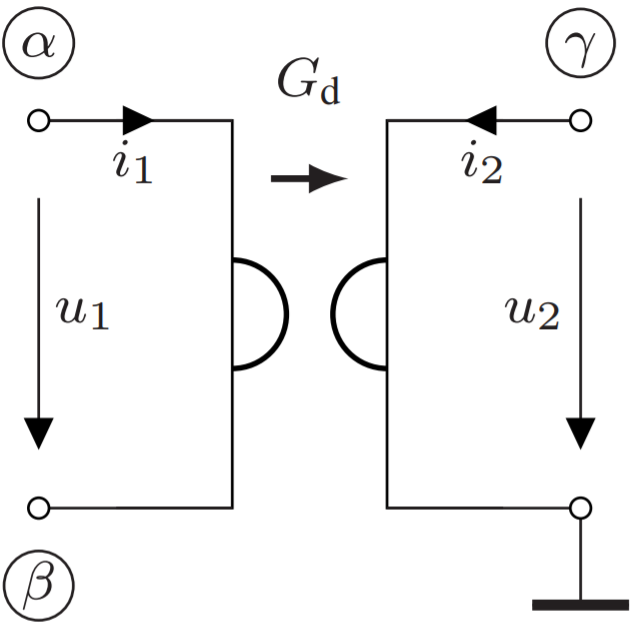
\includegraphics[scale=0.15]{./img/nodevoltageanalysis/gyrator_a_b_y_gnd.png} } \\
        $\ma {Y_k} = \kbordermatrix{ & u_{k\alpha} &                                   & u_{k\gamma}                                                                                    &                                  & u_{k\delta}                                                                                  \\
        \alpha                       &             & \ldots                            & G_d                                                                                            & \ldots                           & -G_d                                                                                         \\
                                     & \vdots      &                                   & \vdots                                                                                         &                                  & \vdots                                                                                       \\
        \gamma                       & -G_d        & \ldots                                                                                                                                                                                                                                                               \\
                                     & \vdots                                                                                                                                                                                                                                                                             \\
        \delta                       & G_d         & \ldots \\}$ & \parbox{3cm}{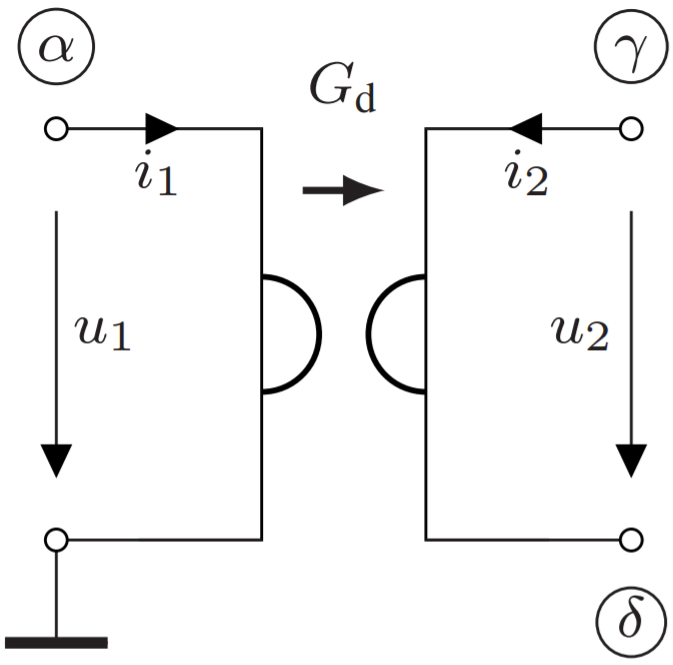
\includegraphics[scale=0.15]{./img/nodevoltageanalysis/gyrator_a_y_d_gnd.png} }                                                                                                                                     \\
        $\ma {Y_k} = \kbordermatrix{ & u_{k\alpha} &                                   & u_{k\gamma}                                                                                                                                                                                                                      \\
        \alpha                       &             & \ldots                            & G_d                                                                                                                                                                                                                              \\
                                     & \vdots      &                                   & \vdots                                                                                                                                                                                                                           \\
        \gamma                       & -G_d        & \ldots\\}$  & \parbox{3cm}{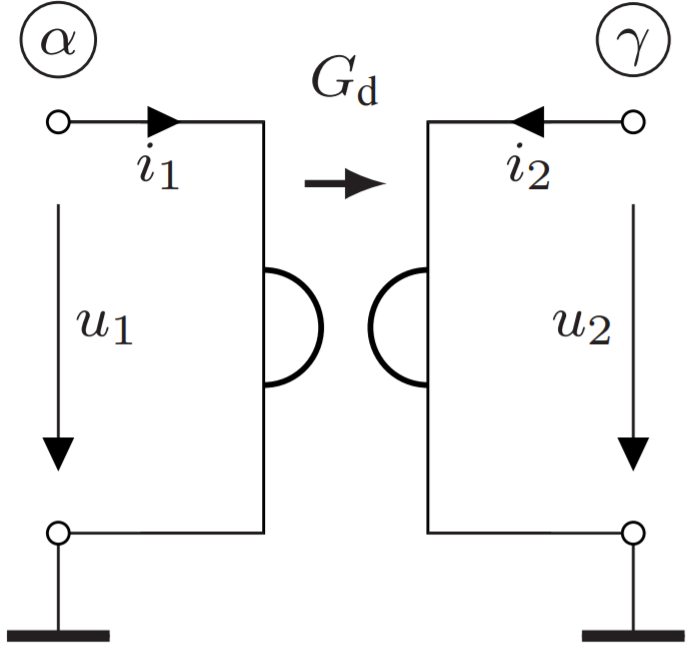
\includegraphics[scale=0.15]{./img/nodevoltageanalysis/gyrator_a_y_gnd_gnd.png} }                                                                                                                                   \\
    \end{tabular}
    $\ \ \ \ \ma {Y_k} = \kbordermatrix{ & u_{k\alpha} & & u_{k\beta} & & u_{k\gamma} & & u_{k\delta}\\
            \alpha & & & & \ldots & G_d & \ldots & -G_d\\
            & & & & & \vdots & & \vdots\\
            \beta & & & & \ldots & -G_d & \ldots & G_d\\
            & \vdots & & \vdots && \vdots && \vdots\\
            \gamma & -G_d & \ldots & G_d & \ldots\\
            & \vdots & & \vdots\\
            \delta & G_d & \ldots & -G_d & \ldots \\}$ \\
    \begin{center}
        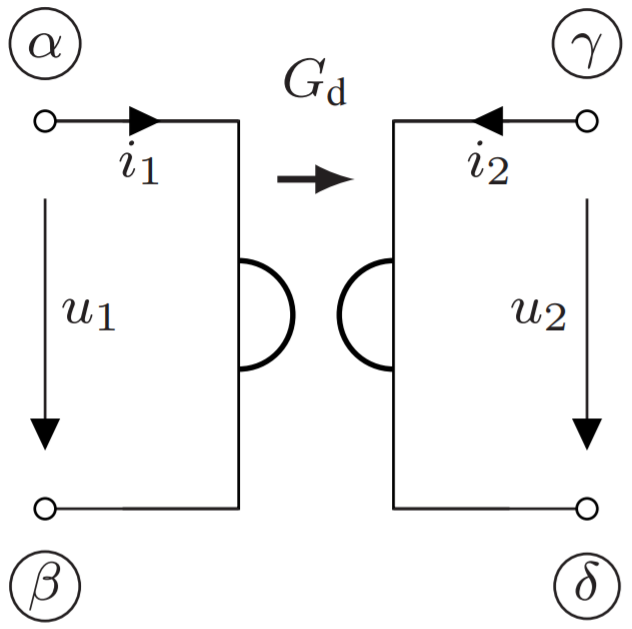
\includegraphics[scale=0.15]{./img/nodevoltageanalysis/gyrator_a_b_y_d.png}
    \end{center}\ \\
    Jeder Gyrator fügt einen weiteren Knoten (und somit ein weiteres Knotenpotenzial) hinzu $\rightarrow Y_k$ wächst um eine Zeile und um eine Spalte.\\
    Bei Dualwandlung kann man Tor 2 des Gyrators \textbf{immer} unten mit Masse verbinden!\\\\
    \hrule
    \begin{tabular}{ll}
        $\ \ \ \ \ma {Y_k} = $
        $\kbordermatrix{ &        & u_{k\alpha} &                            & u_{k\beta}                                                                                   &                                                                                                                         \\
                         &        & \vdots      &                            & \vdots                                                                                       &                                                                                                                         \\
        \alpha           & \ldots & G           & \ldots                     & -G                                                                                           & \ldots                                                                                                                  \\
                         &        & \vdots      &                            & \vdots                                                                                       &                                                                                                                         \\
        \beta            & \ldots & -G          & \ldots                     & G                                                                                            & \ldots                                                                                                                  \\
                         &        & \vdots      &                            & \vdots                                                                                       & \\}$ & \parbox{3cm}{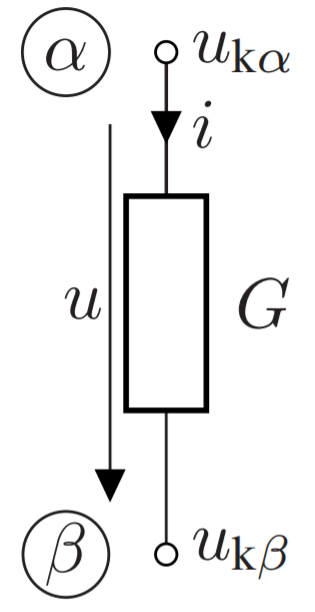
\includegraphics[scale=0.15]{./img/nodevoltageanalysis/conductance_a_b.png} } \\

        $\ \ \ \ \ma {Y_k}$ =
        $\kbordermatrix{ &        & u_{k\alpha} &                                                                                                                                                                                                                                                     \\
                         &        & \vdots      &                                                                                                                                                                                                                                                     \\
        \alpha           & \ldots & G           & \ldots                                                                                                                                                                                                                                              \\
                         &        & \vdots      & \\}$ & \parbox{3cm}{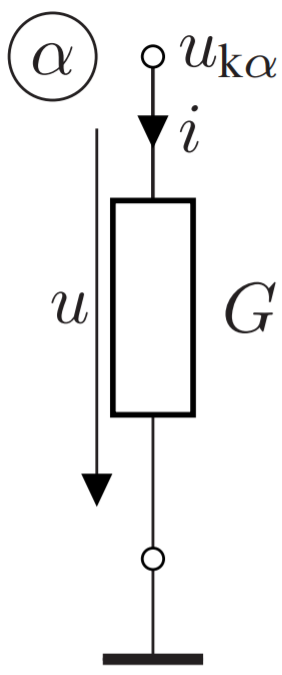
\includegraphics[scale=0.15]{./img/nodevoltageanalysis/conductance_a_gnd.png} }                                                                                                                           \\
    \end{tabular}

    \begin{tabular}{ll}
        $\ \ \ \ \ma {Y_k}$ =
        $\kbordermatrix{ & u_{k\gamma} &                            & u_{k\delta}                                                                                                                                                                                                                                  \\
                         & \vdots      &                            & \vdots                                                                                                 &                                                                                                                                     \\
        \alpha           & g_m         & \ldots                     & -g_m                                                                                                                                                                                                                                         \\
                         & \vdots      &                            & \vdots                                                                                                                                                                                                                                       \\
        \beta            & -g_m        & \ldots                     & g_m                                                                                                                                                                                                                                          \\
                         & \vdots      &                            & \vdots                                                                                                 & \\}$ & \hspace{-2em}\parbox{3cm}{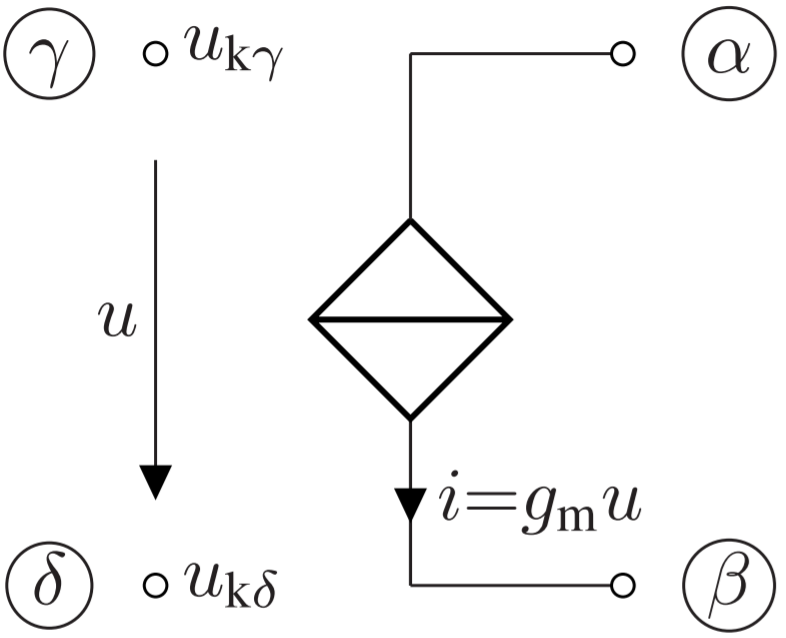
\includegraphics[scale=0.15]{./img/nodevoltageanalysis/vccs_a_b_y_d.png} }   \\

        $\ \ \ \ \ma {Y_k}$ =
        $\kbordermatrix{ & u_{k\gamma} &                                                                                                                                                                                                                                                                           \\
                         & \vdots      &                                                                                                                                                                                                                                                                           \\
        \alpha           & g_m         & \ldots                                                                                                                                                                                                                                                                    \\
                         & \vdots      &                                                                                                                                                                                                                                                                           \\
                         & \vdots      &                                                                                                                                                                                                                                                                           \\
        \beta            & -g_m        & \ldots                                                                                                                                                                                                                                                                    \\
                         & \vdots      & \\}$ & \hspace{-2em}\parbox{3cm}{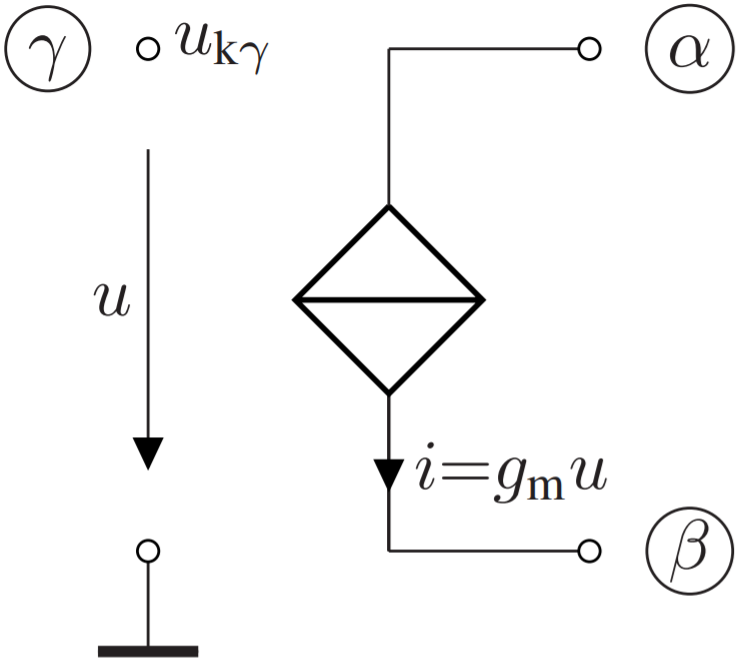
\includegraphics[scale=0.15]{./img/nodevoltageanalysis/vccs_a_b_y_gnd.png} }                                                                                                                                       \\

        $\ \ \ \ \ma {Y_k}$ =
        $\kbordermatrix{ & u_{k\gamma} &                            & u_{k\delta}                                                                                            &                                                                                                                                     \\
                         & \vdots      &                            & \vdots                                                                                                 &                                                                                                                                     \\
        \alpha           & g_m         & \ldots                     & -g_m                                                                                                   & \ldots                                                                                                                              \\
                         & \vdots      &                            & \vdots                                                                                                 & \\}$ & \hspace{-2em}\parbox{3cm}{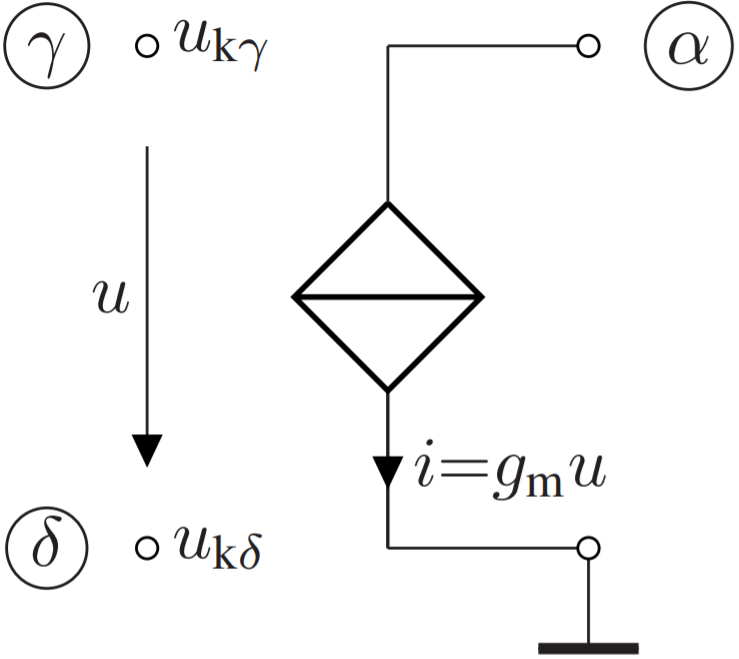
\includegraphics[scale=0.15]{./img/nodevoltageanalysis/vccs_a_y_d_gnd.png} } \\

        $\ \ \ \ \ma {Y_k}$ =
        $\kbordermatrix{ & u_{k\gamma} &                                                                                                                                                                                                                                                                           \\
                         & \vdots      &                                                                                                                                                                                                                                                                           \\
        \alpha           & g_m         & \ldots                                                                                                                                                                                                                                                                    \\
                         & \vdots      & \\}$ & \hspace{-2em}\parbox{3cm}{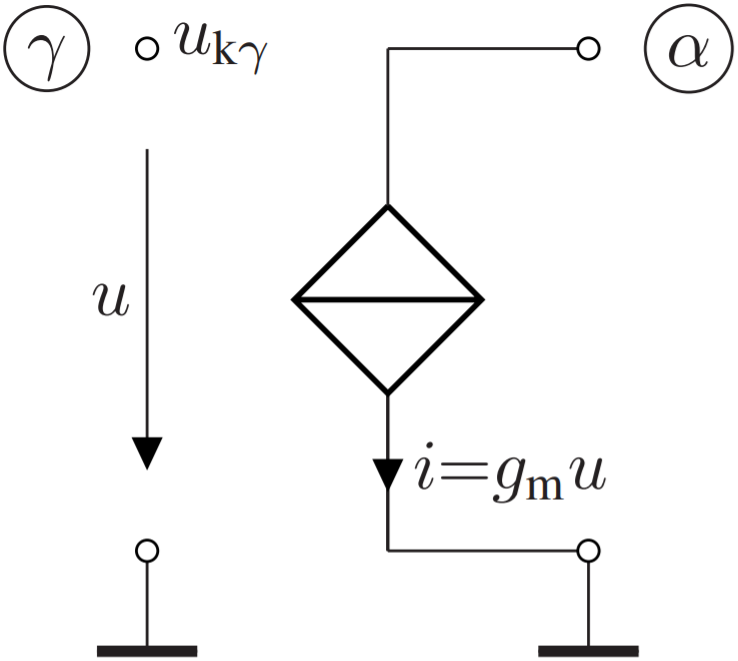
\includegraphics[scale=0.15]{./img/nodevoltageanalysis/vccs_a_y_gnd.png} }                                                                                                                                         \\
    \end{tabular}\\
    Jede Quellwandlung löscht einen Knoten (und somit ein Knotenpotenzial) $\rightarrow Y_k$ schrinkt um eine Zeile und um eine Spalte.\\\\
    \hrule

    \begin{center}
        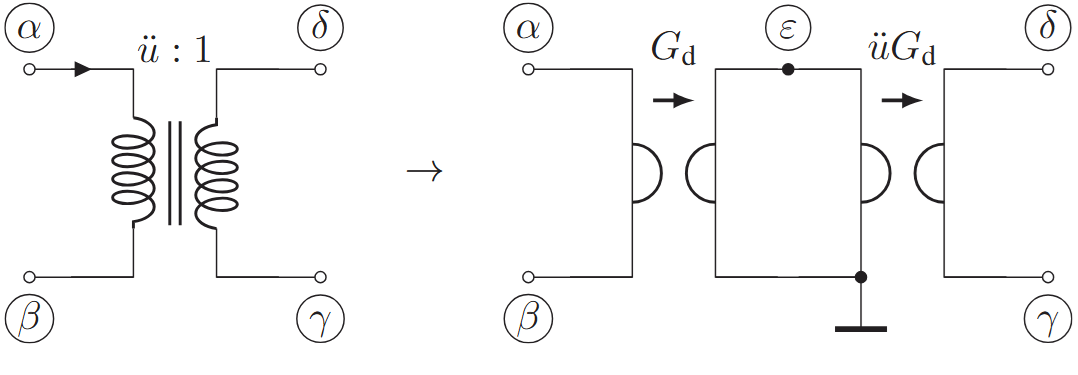
\includegraphics[scale=0.25]{./img/nodevoltageanalysis/transformer_gyrator_model.png}
    \end{center}

    \normalsize

    \sectionbox{
        \subsubsection{Gesteuerte Quellen}
        \begin{itemize}
            \item VCCS: Muss nicht geändert werden
            \item VCVS: Quellwandeln oder dualwandeln $\rightarrow$ VCCS
            \item CCVS: Quellwandeln oder dualwandeln, um CCCS zu erhalten
            \item CCCS:
            \item[-] Steuernden Strom durch Spannungen ausdrücken (nur möglich, wenn man für den steuernden Strom eine Gleichung findet)
            \item[-] Ansonsten muss man den KS (dort wo der steuernde Strom fließt) mithilfe Dualwandlung durch einen LL ersetzen. Dadurch kann man den steuernden Strom durch $G_d u_{Gyr,2}$ ausdrücken
        \end{itemize}
    }

    \subsubsection{Aufstellen des Knotenstromquellenvektors}
    Bei dem Vektor $\vec i_{q}$ werden die \textbf{konstanten Quellenströme} eingetragen.
    Anders als üblicherweise, trägt man in der jeweiligen Zeile des Knotens \textbf{herausfließende} Ströme \textbf{negativ} ein und \textbf{hineinfließende} Ströme \textbf{positiv} ein.\\

    Ist eine Quelle auf einer Seite mit dem Masseknoten verbunden, wird nur der Wert für den gegenüberliegenden (nicht mit Masse verbundenen) Knoten im Stromquellenvektor eingetragen.\\

    Beispiel: Eine Schaltung besitzt 4 Knoten (inklusive Masse) und $I_0$ fließt von Masse in Knoten 2. Der resultierende Vektor $\vec i_q$ lautet:
    \begin{center} % using $$ adds a lot of padding in this template
        $\vec i_{q} = \mat{0 & I_0 & 0}^T$
    \end{center}

    \section{Netzwerkeigenschaften}

    \subsection{Dualwandlung}
    $\vec u \xrightarrow{R_d} R_d\vec i^d$\qquad$\vec i \xrightarrow{R_d} \frac{1}{R_d}\vec u^d$\\
    $\ma A\vec i = \vec 0 \xrightarrow{R_d} \ma A\vec u^d = \vec 0$ Knoten werden zu Maschen\\
    $\ma B\vec u = \vec 0 \xrightarrow{R_d} \ma B\vec i^d = \vec 0$ Maschen werden zu Knoten\\
    \begin{tabular}{cc}
        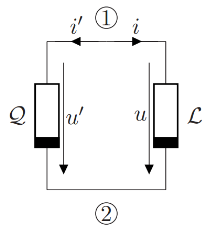
\includegraphics[width=.295\columnwidth]{img/dual_start} &
        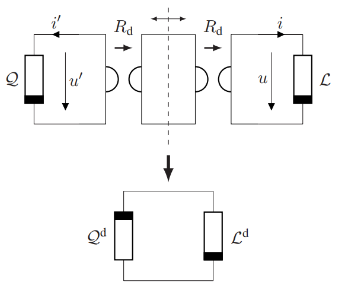
\includegraphics[width=.595\columnwidth]{img/dual_end}
    \end{tabular}
    $\mat{\vec u^d\\\vec i^d}=\mat{0&R_d\\\frac{1}{R_d}&0}\mat{\vec u\\\vec i}$

    \subsection{Substitutionstheorem}
    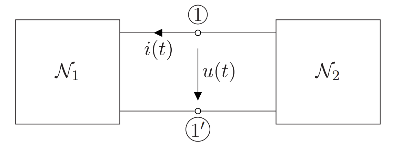
\includegraphics[scale=.27]{img/subst}\\
    \begin{tabular}{cc}
        \multicolumn{2}{c}{Wenn $\mathcal N_1$ zu allen Zeitpunkten} \\
        spannungsgestuert                        & stromgesteuert    \\
        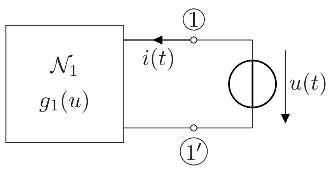
\includegraphics[scale=.25]{img/subst-u} &
        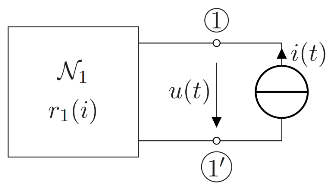
\includegraphics[scale=.25]{img/subst-i}
    \end{tabular}

    \sectionbox{
        \subsection{Zweipolersatzschaltungen}
        Eine beliebe Eintorschaltung $\mathcal F$ aus linearen resistiven
        Netzwerkelementen lässt sich durch mindestens eine
        der beiden folgenden Ersatzeintore beschreiben.\\
        \begin{tabular}{cc}
            \textbf{Helmholz / Thévenin ESB}                          &
            \textbf{Mayer / Norton ESB}                                                        \\
            \hspace{-1.5em}\begin{circuitikz}
                               \draw (0,0) to[R, l=R, i_<=$i$, -o] (2,0);
                               \draw (2,-2) to[short, o-] (0, -2) to[V, v<=$U_0$] (0,0);
                               \draw (2,0) to[open, v^>=$u$] (2, -2);
                           \end{circuitikz} &
            \hspace{-.5em}\begin{circuitikz}
                              \draw (0,0) -- (1,0) to[short, i^<=$i$, -o] (2,0);
                              \draw (2, -2) to[short, o-] (1, -2) --(0, -2) to[I, i<^=$I_0$] (0,0);
                              \draw (1,0) to[R, l = G] (1, -2);
                              \draw (2,0) to[open, v^>=$u$] (2,-2);
                          \end{circuitikz} \\
        \end{tabular}\\
        Umrechnung durch Quellwandlung:\\
        $\begin{array}{lcl}
                R_i = \frac{1}{G_i}    & \Leftrightarrow & G_i=\frac{1}{R_i}    \\
                u_0 = -\frac{i_0}{G_i} & \Leftrightarrow & i_0=-\frac{u_0}{R_i}
            \end{array}$
        \textbf{Bestimmen von $u_0$/$i_0$}: Leerlaufspannung bzw. Kurzschlussstrom von $\mathcal F$ bestimmen\\
        \textbf{Bestimmen von $R_i$/$G_i$}: Unabhängige Quellen in $\mathcal F$ durch entsprechende Nullquellen ersetzen und dann eine Torgröße in Abhängigkeit der anderen bestimmen.
    }

    \columnbreak

    \section{Allgemeines Reaktiver Elemente}
    % ===============================================================================================

    \subsection{Die vier zentralen Zustandsgrößen $u,i,q,\Phi$}
    % ----------------------------------------------------------------------
    ... beschreiben die Wirkungsweise von elektronischen Bauelementen.\\ \\
    \textbf{Spannung \textit{u}}: Potentialdifferenz. Hohes zu niedrigem Potential\\
    \textbf{Strom \textit{i}}: Bewegte Ladung. Bewegungsrichtung positiver Ladung\\
    \textbf{Ladung \textit{q}}: Grundeigenschaft von Materie.\\
    \textbf{Magnetischer Fluss \textit{$\Phi$}}: Grundeigenschaft von elektr. magn. Feldern\\
    \subsubsection{Allgemeine Zusammenhänge $u,i,q,\Phi$}
    \textbf{Kondensator} ist u-gesteuert (q-gesteuert), falls für ein u (q) nur ein q (u)  existiert: $q=c(u)$ ($u=\chi(q)$) \\
    \textbf{Induktivität} ist i-gesteuert ($\Phi$-gesteuert), falls für ein i ($\Phi$) nur ein $\Phi$ (i) existiert: $\Phi=l(i)$ ($i=\lambda(\Phi)$) \\
    \sectionbox{
        \begin{tabular}{l|l}
            $i(t) = \dot q(t)$                                         & $[i]=A$        \\
            $q(t) = q(t_0) + \int_{t_0}^t i(\tau) \mathrm d\tau$       & $[q]=As=C$     \\ \hline
            $u(t) = \dot \Phi(t)$                                      & $[u]=V$        \\
            $\Phi(t) = \Phi(t_0) + \int_{t_0}^t u(\tau) \mathrm d\tau$ & $[\Phi]=Vs=Wb$ \\
        \end{tabular}\\
    }


    \subsubsection{Arten von Bauelementen}
    \begin{tabular}{l|l|l|l}
        Art           & Symbol                                                  & Beschr.       & linear                \\ \hline
        Resistivität  & 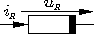
\includegraphics[height=0.4cm]{./img/Resistivitat.pdf}  & $f_R(u,i)$    & $u = U_0 + R i$       \\
        Kapazität     & 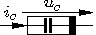
\includegraphics[height=0.4cm]{./img/Kapazivitat.pdf}   & $f_C(u,q)$    & $q = Q_0 + C u$       \\
                      &                                                         &               & $i(t)=C\dot u(t)$     \\
                      &                                                         &               & $[C]=\frac{As}{V}=F$  \\
        Induktivität  & 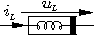
\includegraphics[height=0.4cm]{./img/Induktivitat.pdf}  & $f_L(i,\Phi)$ & $\Phi = \Phi_0 + L i$ \\
                      &                                                         &               & $u(t)=L\dot i(t)$     \\
                      &                                                         &               & $[L]=\frac{Wb}{A}=H$  \\
        Memristivität & 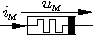
\includegraphics[height=0.4cm]{./img/Memristivitat.pdf} & $f_M(q,\Phi)$ & $\Phi = \Phi_0 + M q$ \\
    \end{tabular}
    \subsubsection{Zusammenhang der Bauelemente}
    \begin{center}
        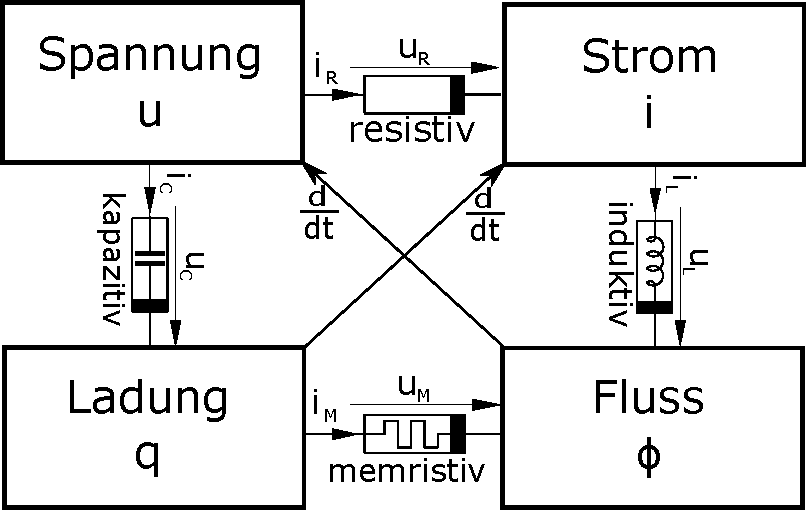
\includegraphics[scale=0.3]{./img/reactance_overview.pdf}
    \end{center}
    \sectionbox{
        \subsubsection{Eigenschaften von Reaktanzen}
        \textbf{Linearität}: siehe Eintore\\
        \textbf{Gedächtnis}: Verhalten durch vorhergehende Klemmengrößen bestimmt.\\
        \textbf{Stetigkeit}: $u_C(t)$, $i_L(t)$ stetig in $(t_a, t_b)$, wenn Torgrößen endlich\\
        Zustandsgrößen (welche auch die Integralgrößen sind) der jeweiligen Elemente sind stetig. Ladung und Spannung sind bei der Kapazität stetig (Zustandsgrößen der Kapazität), Strom und Fluss nicht unbedingt. Bei Induktivitäten andersrum.\\
        \textbf{Verlustfreiheit}: $W_C(t_1, t_2) = \int_{t_1}^{t_2}\! u(t)i(t)\,\mathrm dt = \int_{q(t_1)}^{q(t_2)}\! \chi(q)\,\mathrm{d}q=W_C(q(t_1), q(t_2))$ (Arbeit)\\
        Falls linear: $W = \frac{Cu^2}{2} = \frac{Li^2}{2}$\\
        Periodisch: $u(t+T) = u(t)$, $q(t+T) = q(t)$\\
        Graphisch: Falls keine geschlossenen Schleifen in q/u, $\Phi$/i-Diagramm existiert (Hysteresefrei) bzw. falls sie in jedem Punkt der Kennlinie gesteuert ist (kann auch in einem Teil spannungs- und in anderem Teil ladungsgest. sein): Normale Linie $\rightarrow$ verlustlos\\
    }

    \sectionbox{
        \subsubsection{Energie und Arbeit}
        \textbf{Arbeit (nicht linearer Fall)}:
        \begin{enumerate}
            \item[-] Kapazitiv: $W_C(t_1, t_2) = \int_{t_1}^{t_2} \! u(t)i(t)\, \mathrm dt = \int_{q_1}^{q_2} \! \chi(q)\, \mathrm dq$, $u=\chi(q)$
            \item[-] Induktiv: $W_L(t_1, t_2) = \int_{t_1}^{t_2} \! u(t)i(t)\, \mathrm dt = \int_{\Phi_1}^{\Phi_2} \! \lambda(\Phi)\, \mathrm d\Phi$, $i=\lambda(\Phi)$
        \end{enumerate}
        \textbf{Arbeit (linearer Fall)}:
        \begin{enumerate}
            \item[-] Kapazitiv: $W_C(q_1,q_2)=\frac{C}{2}(u_2^2-u_1^2)=\frac{1}{2C}(q_2^2-q_1^2)$
            \item[-] Induktiv: $W_L(\Phi_1,\Phi_2)=\frac{L}{2}(i_2^2-i_1^2)=\frac{1}{2L}(\Phi_2^2-\Phi_1^2)$
        \end{enumerate}
        \textbf{Energie (linearer Fall)}:
        \begin{enumerate}
            \item[-] Kapazitiv: $W_C = \frac{C}{2}u^2 = \frac{1}{2C}q^2$
            \item[-] Induktiv: $W_L = \frac{L}{2}i^2 = \frac{1}{2L} \Phi^2$
        \end{enumerate}
        Graphisch: Fläche zwischen der Kennlinie und der q-/$\Phi$-Achse\\
        \textbf{Relaxationspunkte (=Ruhepunkte)}: Betriebspunkte, in dem die in einer Reaktanz gespeicherte Energie minimal ist. Kandidaten sind: Extremwerte, Wendepunkte, Knicke, Schnittpunkte mit q-/$\Phi$-Achse\\
    }

    \subsubsection{Verschaltung von Reaktanzen}
    - Parallelschaltung: $C_p = C_1 + C_2$, $L_p = L_1 || L_2 = \frac{L_1L_2}{L_1+L_2}$\\
    - Serienschaltung: $C_p = C_1 || C_2 = \frac{C_1C_2}{C_1+C_2}$, $L_p = L_1 + L_2$\\


    Merke: Am Kondensa\textsl{tor}, eilt der Strom \textsl{vor}, bei Induktivi\textsl{täten}, wird er sich ver\textsl{späten}\\

    \subsubsection{Dualwandlung}
    $u \rightarrow R_d i^d$\qquad
    $i \rightarrow \frac{1}{R_d} u^d$\qquad
    $\Phi \rightarrow R_d q^d$\qquad
    $q \rightarrow \frac{1}{R_d}\Phi^d$\\
    $C^d \rightarrow \frac{L}{R_d^2}$ \qquad $L^d \rightarrow R_d^2C$

    \section{Komplexe Wechselstromrechnung}
    Vorraussetzung: lineares, eingeschwungenes System mit sinusförmiger Erregung $a(t) = A_m \cos(\omega t + \varphi)$\\
    \sectionbox{
        \subsection{Komplexe Zeigergrößen}
        \emphbox{
            \begin{tabular}{ll}
                \textbf{Zeitfunktion} & $a(t) = A_m\cos(\omega t+\phi)=\Re{Ae^{j\omega t}}$ \\
                \textbf{Zeiger}       & \parbox{3cm}{\begin{align*}
                                                             A & = \alpha + j\beta = A_m  e^{j\phi} \\
                                                               & = A_m  (\cos \phi+j\sin \phi)
                                                         \end{align*}} \\
                \textbf{Maximum}      & $A_m = |A| = \sqrt{\alpha^2+\beta^2} = \sqrt{AA^*}$ \\
                \textbf{Phase}        & $\phi = \begin{cases}
                                                        \arctan\frac{\beta}{\alpha}     & \alpha>0 \\
                                                        \arctan\frac{\beta}{\alpha}+\pi & \alpha<0 \\
                                                    \end{cases}$  \\\\
                \textbf{Kapazität}    & $I_C=j\omega CU_C$                                  \\
                \textbf{Induktivität} & $U_L=j\omega LI_L$
            \end{tabular}
        }

        % ---------------------------------------------------------
        Differentialoperator: $\frac{\diff}{\diff t} = j \omega$\qquad
        $\frac{d}{dt} e^{j(\omega t + \phi)} = j\omega e^{j(\omega t + \phi)} \rightarrow \dot u(t)=j\omega U$\\
        Kreisfrequenz: $\omega = 2\pi f = \frac{2\pi}{T}$\\
        \tablebox{
            \begin{tabular*}{\columnwidth}{l@{\extracolsep\fill}cccc} \ctrule
                & \textbf{Widerstand} & \textbf{Kondensator} & \textbf{Spule} & \textbf{Memristor}\\ \cmrule
                $\frac{U}{I} =$ & $R$ & $\frac{1}{j \omega C}$ & $j \omega L$ & $M$\\[0.5em]
                $\underset{\varphi_u - \varphi_i}{\Delta \varphi =}$ & 0 & $-\frac{\pi}{2}$ & $\frac{\pi}{2}$ & ?\\ \cbrule
            \end{tabular*} }
    }

    \sectionbox{
        \subsection{Netzwerkgleichungen}
        Gleichungssysteme kann man analog zu resistiven Netzwerken mithilfe Zeigergrößen aufstellen:
        \begin{itemize}
            \item $\ma A \vec i= \vec 0 \rightarrow \ma A \vec  I = \vec 0 \qquad \vec i(t)=\Re{\vec I e^{j\omega t}}$
            \item $\ma B \vec u= \vec 0 \rightarrow \ma B \vec  U = \vec 0 \qquad \vec u(t)=\Re{\vec U e^{j\omega t}}$
            \item $\ma A^T \vec u_k= \vec u \rightarrow \ma A^T \vec  U_k = \vec U \qquad \vec u_k(t)=\Re{\vec U_k e^{j\omega t}}$
        \end{itemize}

        \subsubsection{Netzwerkelemente in Zeigerdarstellung}
        Elemente werden in Zeigerdarstellung umgeschrieben und dann genauso wie in resistiven Netzwerken in das Tableau-Gleichungssystem eingesetzt. Für Kapazitäten und Induktivitäten ergibt sich somit ein extra $j\omega$ in dem jeweiligen Feld\\
        $\ma M(j \omega) = j\omega \ma M_1 + \ma M_0 \qquad \ma N(j\omega) = j\omega \ma N_1 + N_0$
    }

    \sectionbox{
        \subsection{Komplexe Leistungsrechnung}
        $U_{eff} = \frac{1}{\sqrt{2}}U_m$\quad
        $I_{eff} = \frac{1}{\sqrt{2}}I_m$\\
        \textbf{Momentanleistung}: $p(t) = u(t)i(t)$\\
        \textbf{Energie einer Periode}: $E=\int_0^Tu(t)i(t)dt=P_WT$\\
        \textbf{Leistungsmittelwert}: $P_w = \frac{1}{T} \int_0^T u(t)i(t)dt$\\
        \textbf{Komplexe Leistung}: $P = \frac{1}{2}UI^* = \frac{1}{2}U_m e^{j\phi_u} I_m e^{-j\phi_i} = U_{eff} I_{eff} e^{j(\phi_u-\phi_i)}$\\
        \textbf{Scheinleistung}: $S = |P|$\\
        \textbf{Wirkleistung}: $P_w = \Re{P}$\\
        \textbf{Blindleistung}: $P_B = \Im{P}$
    }

    \sectionbox{
        \textbf{Superpositionsprinzip}\\
        Superpositionsprinzip gilt \textbf{NUR} im Zeitbereich. Mann muss die Schaltung also bei mehreren $\omega$s separat analysieren, die Zeiger in $a_i(t)=\Re{A_ie^{j\omega}t}$ umwandeln, und dann $a_1(t)+a_2(t)+...$ addieren.
    }

    \section{Mathe}
    \sectionbox{
        \subsection{Matrizen}
        \subsubsection{2x2 Matrizen}
        $\det\mat{a&b\\c&d} = ad-bc$\qquad
        $\begin{bmatrix}
                a & b \\c&d
            \end{bmatrix}^{-1} =\frac{1}{ad-bc} \begin{bmatrix}
                d & -b \\-c&a
            \end{bmatrix}$

        \subsubsection{Cramer'sche Regel}
        Für ein lineares Gleichungssystem $\ma A  \vec x = \vec y$ gilt:
        \[x_i=\frac{\det \ma A_i}{\det \ma A}\]
        wobei $\ma A_i$ aus $\ma A$ entsteht, wenn man die $i$-te Spalte mit dem Vektor $\vec y$ ersetzt.
    }

    \sectionbox{
        \subsection{Raumdarstellungen}
        Parametrische Beschreibung:\\
        $Bild\begin{bmatrix}
                \ma U \\ \ma I
            \end{bmatrix} = \left\{\begin{bmatrix}
                \vec u \\ \vec i
            \end{bmatrix}|\begin{bmatrix}
                \vec u \\ \vec i
            \end{bmatrix}=\begin{bmatrix}
                \ma U \\ \ma I
            \end{bmatrix}\vec c,\vec c \in R^p \right\}$\\
        Implizite Beschreibung:\\
        $Kern\mat{\ma U&\ma I} = \left\{\mat{\vec u\\ \vec i}|\mat{\ma M&\ma N}\mat{\vec u\\\vec i}=0\right\}$\\
        ($\mat{\ma M&\ma N}$ implizite Beschreibung des lin. Zweitors)
    }

    \sectionbox{
        \subsection{Integration}
        \begin{tabular}{l|l}
            $a$                       & $a x$                        \\
            $e^{x}$                   & $e^{x}$                      \\
            $\ln(x)$                  & $x\ln(x)-x$                  \\
            $\frac{1}{x}$             & $\ln\left|x\right|$          \\
            $\sqrt[n]{x}=x^{\frac1n}$ & $\frac{n}{n+1}x^{\frac1n+1}$ \\
        \end{tabular}
    }

    \sectionbox{
        \subsection{Trigonometrie}
        $\cos(x) = \cos(-x)$\\
        $\sin(-x) = -\sin(x)$\\
        $\sin^2(x) + \cos^2(x) = 1$\\
        $\cos(x) = \sin\left(x + \frac{\pi}{2}\right)$\\
        $\sin(x) = \cos\left(x - \frac{\pi}{2}\right)$\\
        $\cos(x+y) = \cos(x)\cos(y) - \sin(x)\sin(y)$\\
        $\sin(x+y) = \sin(x)\cos(y) + \cos(x)\sin(y)$\\
        $\tan(x) = \frac{\sin(x)}{\cos(x)} \in[-1,1]$\\
        $\arctan(x) \in\left(-\frac{\pi}{2}, \frac{\pi}{2}\right)$\\

        % Credit:
        % https://tex.stackexchange.com/questions/637299/draw-trigonometric-circle-with-tikz-package
        \definecolor{col_sectionbox}{RGB}{251, 251, 251} % for some reason the color macros from the template don't work
        \textbf{Wichtige Sinus- und Cosinuswerte} $(\cos x, \sin x)$\\
        \begin{tikzpicture}[scale=1.8,
                cap = round,
                > = latex,
                dot/.style = {circle, fill, minimum size=1.2mm},
                lbl/.style = {fill=col_sectionbox, inner sep=2pt, near start, sloped}
            ]
            % draw the coordinates
            \draw[->] (-1.5,0) -- (1.7,0) node[right] {$x$};
            \draw[->] (0,-1.5) -- (0,1.5) node[above] {$y$};
            % draw the unit circle
            \draw[thick] (0,0) circle[radius=1];
            % draw dots, labels
            \foreach \i/\j/\k in {
            30/\frac{\pi}{6}/{\left(\frac{\sqrt{3}}{2},\frac{1}{2}\right)},
            45/\frac{\pi}{4}/{\left(\frac{\sqrt{2}}{2},\frac{\sqrt{2}}{2}\right)},
            60/\frac{\pi}{3}/{\left(\frac{1}{2},\frac{\sqrt{3}}{2}\right)},
            90/\frac{\pi}{2}/{\rotatebox{-90}{(0,1)}},
            120/\frac{2\pi}{3}/{\left(\frac{-1}{2},\frac{\sqrt{3}}{2}\right)},
            135/\frac{3\pi}{4}/{\left(\frac{-\sqrt{2}}{2},\frac{\sqrt{2}}{2}\right)},
            150/\frac{5\pi}{6}/{\left(\frac{-\sqrt{3}}{2},\frac{1}{2}\right)},
            180/\pi/{(-1,0)},
            210/\frac{7\pi}{6}/{\left(\frac{\sqrt{3}}{2},\frac{-1}{2}\right)},
            225/\frac{5\pi}{4}/{\left(\frac{-\sqrt{2}}{2},\frac{-\sqrt{2}}{2}\right)},
            240/\frac{4\pi}{3}/{\left(\frac{-1}{2},\frac{-\sqrt{3}}{2}\right)},
            270/\frac{3\pi}{2}/{\rotatebox{90}{(0,-1)}},
            300/\frac{5\pi}{3}/{\left(\frac{1}{2},\frac{-\sqrt{3}}{2}\right)},
            315/\frac{7\pi}{4}/{\left(\frac{\sqrt{2}}{2},\frac{-\sqrt{2}}{2}\right)},
            330/\frac{11\pi}{6}/{\left(\frac{\sqrt{3}}{2},-\frac{1}{2}\right)},
            360/2\pi/{(1,0)}
            }
            {
            \path[draw=gray]    (\i:0) -- (\i:0.4)
            -- node[lbl] {\tiny $\i^{\circ}$} (\i:0.77)
            -- node[lbl] {$\j$} (\i:1) node[dot] {};
            \ifnum\i<270
                \ifnum\i>90
                    \path   (\i:1) --  node[lbl, anchor=east] {$\k$} (\i:1.4);
                \else
                    \path   (\i:1) --  node[lbl, anchor=west] {$\k$} (\i:1.4);
                \fi
            \else
                \path   (\i:1) --  node[lbl, anchor=west] {$\k$} (\i:1.3);
            \fi
            }
        \end{tikzpicture}
    }
    \sectionbox{
        \subsection{Komplexe Zahlen}
        \textbf{Kartesische Darstellung}: $z = a + j b$\\
        \textbf{Polarkoordinaten}: $z = r  e^{j \varphi}$\\

        Umrechnung:\\
        $r = \sqrt{a^2 + b^2}$, $\varphi = \begin{cases}
                \arctan\frac{b}{a}     & a>0            \\
                \arctan\frac{b}{a}+\pi & a<0 \wedge b>0 \\
                \arctan\frac{b}{a}-\pi & a<0 \wedge b<0
            \end{cases}$\\
        $a = r  \cos(\varphi)$, $b = r  \sin(\varphi)$\\

        \textbf{Real-} und \textbf{Imaginärteil}: $\Re z = a$, $\Im z = b$\\

        \textbf{Euler'sche Formel}: $e^{j \varphi} = \cos(\varphi) + j \sin(\varphi)$\\

        \textbf{Komplexe Konjugation}: $z = a + jb \iff z^* = a - j b$\\
        Distributivität: $(z_1+z_2)^*=z_1^*+z_2^*\qquad (z_1z_2)^*=z_1^*z_2^*$\\
        Konjugation in Polardarstellung: $(r e^{j\varphi})^* = r e^{-j\varphi}$\\

        \textbf{Betrag}: $|z| = |a+jb| = \sqrt{a^2+b^2}\qquad zz^* = |z|^2$\\

        \textbf{Erweitern mit Komplex Konjugiertem}:\\
        \[
            \frac{x}{a+jb} = \frac{x(a-jb)}{a^2+b^2} = \frac{ax}{a^2+b^2} - j\frac{bx}{a^2+b^2}
        \]
    }

    \section{Umrechnung von Zweitormatrizen}
    \textbf{Explizit $\ra$ Explizit}\\
    {
    \setlength{\tabcolsep}{30pt}
    \renewcommand{\arraystretch}{1.3}
    \def\mrule{\noalign{\vspace{5pt}\hrule\vspace{7pt}}}                        % middle rule
    \arraycolsep=3pt
    \tabcolsep=5pt
    \renewcommand{\frac}{\dfrac}
    \rotatebox{270}{
        \begin{tabular}{ccccccc}    % {c|c|c|c|c|c|c}    %
            In $\rightarrow$ & $\ma R$                            & $\ma G$    & $\ma H$ & $\ma H'$ & $\ma A$ & $\ma A'$ \\ \mrule
            $\ma R$          & $\mat{r_{11}                       & r_{12}                                               \\ r_{21} & r_{22} }$ & $\frac{1}{\det \ma G} \mat{ g_{22} & -g_{12} \\ -g_{21} & g_{11} }$ & $\frac{1}{h_{22}} \mat{ \det \ma H & h_{12} \\ -h_{21} & 1 }$ & $\frac{1}{h'_{11}} \mat{ 1 & -h'_{12} \\ h'_{21} & \det \ma H' }$ & $\frac{1}{a_{21}} \mat{ a_{11} & \det \ma A \\ 1 & a_{22} }$ & $\frac{1}{a'_{21}} \mat{ a'_{22} & 1 \\ \det \ma A' & a'_{11} }$ \\ \mrule
            $\ma G$          & $\frac{1}{\det \ma R} \mat{ r_{22} & -r_{12}                                              \\ -r_{21} & r_{11} }$ & $\mat{g_{11} & g_{12} \\ g_{21} & g_{22} }$ & $\frac{1}{h_{11}} \mat{ 1 & -h_{12} \\ h_{21} & \det \ma H }$ & $\frac{1}{h'_{22}} \mat{ \det \ma H' & h'_{12} \\ -h'_{21} & 1 }$ & $\frac{1}{a_{12}} \mat{ a_{22} & -\det \ma A \\ -1 & a_{11} }$ & $\frac{1}{a'_{12}} \mat{ a'_{11} & -1 \\ -\det \ma A' & a'_{22} }$ \\ \mrule
            $\ma H$          & $\frac{1}{r_{22}} \mat{ \det \ma R & r_{12}                                               \\ -r_{21} & 1 }$ & $\frac{1}{g_{11}} \mat{ 1 & -g_{12} \\ g_{21} & \det \ma G }$ & $\mat{h_{11} & h_{12} \\ h_{21} & h_{22} }$ & $\frac{1}{\det \ma H'} \mat{ h'_{22} & -h'_{12} \\ -h'_{21} & h'_{11} }$ & $\frac{1}{a_{22}} \mat{ a_{12} & \det \ma A \\ -1 & a_{21} }$ & $\frac{1}{a'_{11}} \mat{ a'_{12} & 1 \\ -\det \ma A' & a'_{21} }$ \\ \mrule
            $\ma H'$         & $\frac{1}{r_{11}} \mat{ 1          & -r_{12}                                              \\ r_{21} & \det \ma R }$ & $\frac{1}{g_{22}} \mat{ \det \ma G & g_{12} \\ -g_{21} & 1 }$ & $\frac{1}{\det \ma H} \mat{ h_{22} & -h_{12} \\ -h_{21} & h_{11} }$ & $\mat{h'_{11} & h'_{12} \\ h'_{21} & h'_{22} }$ & $\frac{1}{a_{11}} \mat{ a_{21} & -\det \ma A \\ 1 & a_{12} }$ & $\frac{1}{a'_{22}} \mat{ a'_{21} & -1 \\ \det \ma A' & a'_{12} }$ \\ \mrule
            $\ma A$          & $\frac{1}{r_{21}} \mat{ r_{11}     & \det \ma R                                           \\ 1 & r_{22} }$ & $\frac{1}{g_{21}} \mat{ -g_{22} & -1 \\ -\det \ma G & -g_{11} }$ & $\frac{1}{h_{21}} \mat{- \det \ma H & -h_{11} \\ -h_{22} & -1 }$ & $\frac{1}{h'_{21}} \mat{1 & h'_{22} \\ h'_{11} & \det \ma H' }$ & $\mat{a_{11} & a_{12} \\ a_{21} & a_{22} }$ & $\frac{1}{\det \ma A'} \mat{ a'_{22} & a'_{12} \\ a'_{21} & a'_{11} }$ \\ \mrule
            $\ma A'$         & $\frac{1}{r_{12}} \mat{r_{22}      & \det \ma R                                           \\ 1 & r_{11}}$ & $\frac{1}{g_{12}} \mat{-g_{11} & -1 \\ -\det \ma G & -g_{22}}$ & $\frac{1}{h_{12}} \mat{1 & h_{11} \\ h_{22} & \det \ma H}$ & $\frac{1}{h'_{12}} \mat{-\det \ma H' & -h'_{22} \\ -h'_{11} & -1}$ & $\frac{1}{\det \ma A} \mat{a_{22} & a_{12} \\ a_{21} & a_{11} }$ & $\mat{a'_{11} & a'_{12} \\ a'_{21} & a'_{22} }$\\
        \end{tabular}
    }
    }

    \columnbreak
    % ----------------------------------------------------------
    % Systemtheorie -----------------------------
    % ----------------------------------------------------------
    % ----------------------------------------------------------

    \section{Systeme ersten Grades}
    \sectionbox{
    \textbf{I. Resistives ESB bestimmen}\\
    \tablebox{
        \begin{tabular*}{\columnwidth}{@{\extracolsep\fill}l|ll@{}} \trule
            & Kapazität & Induktivität \\ \mrule
            ESB-Typ & Helmholtz-Thévenin & Mayer-Norton\\
            &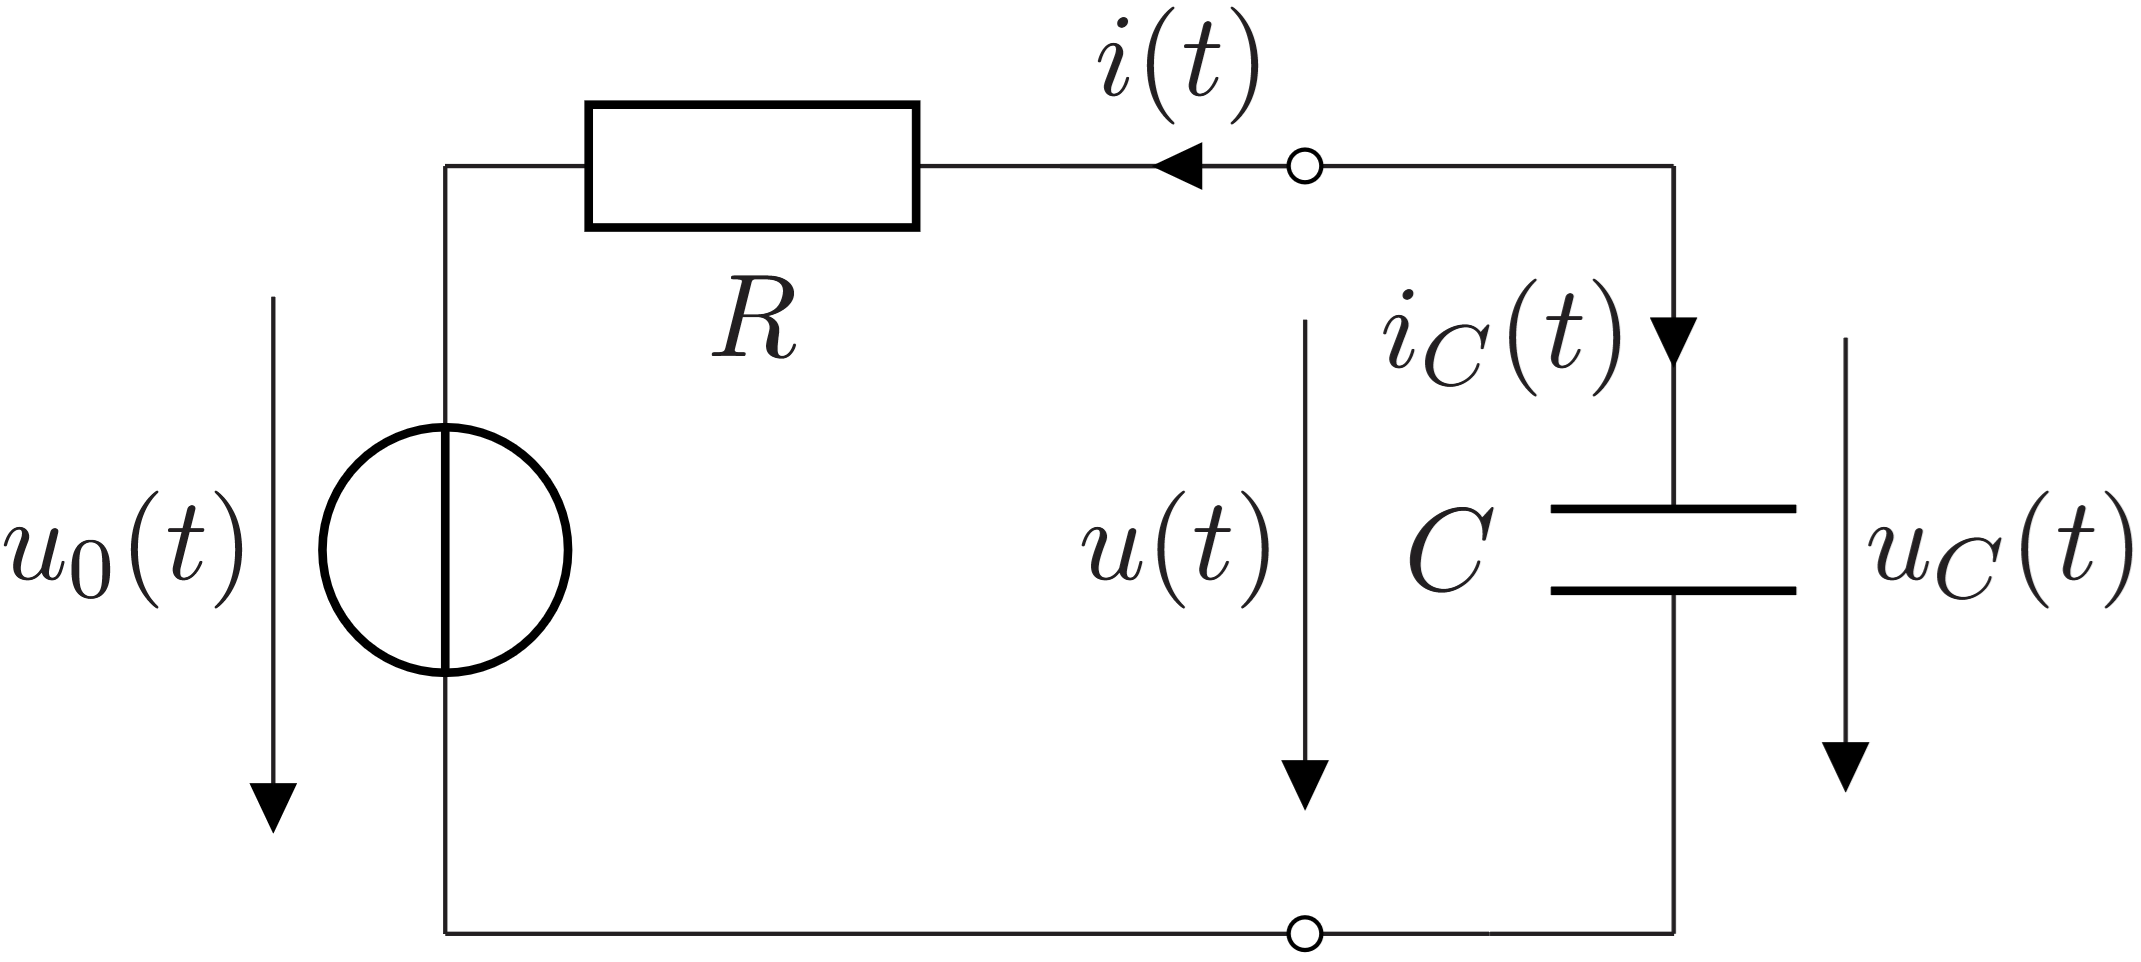
\includegraphics[width=.35\linewidth]{img/helmholtz-thevenin}&
            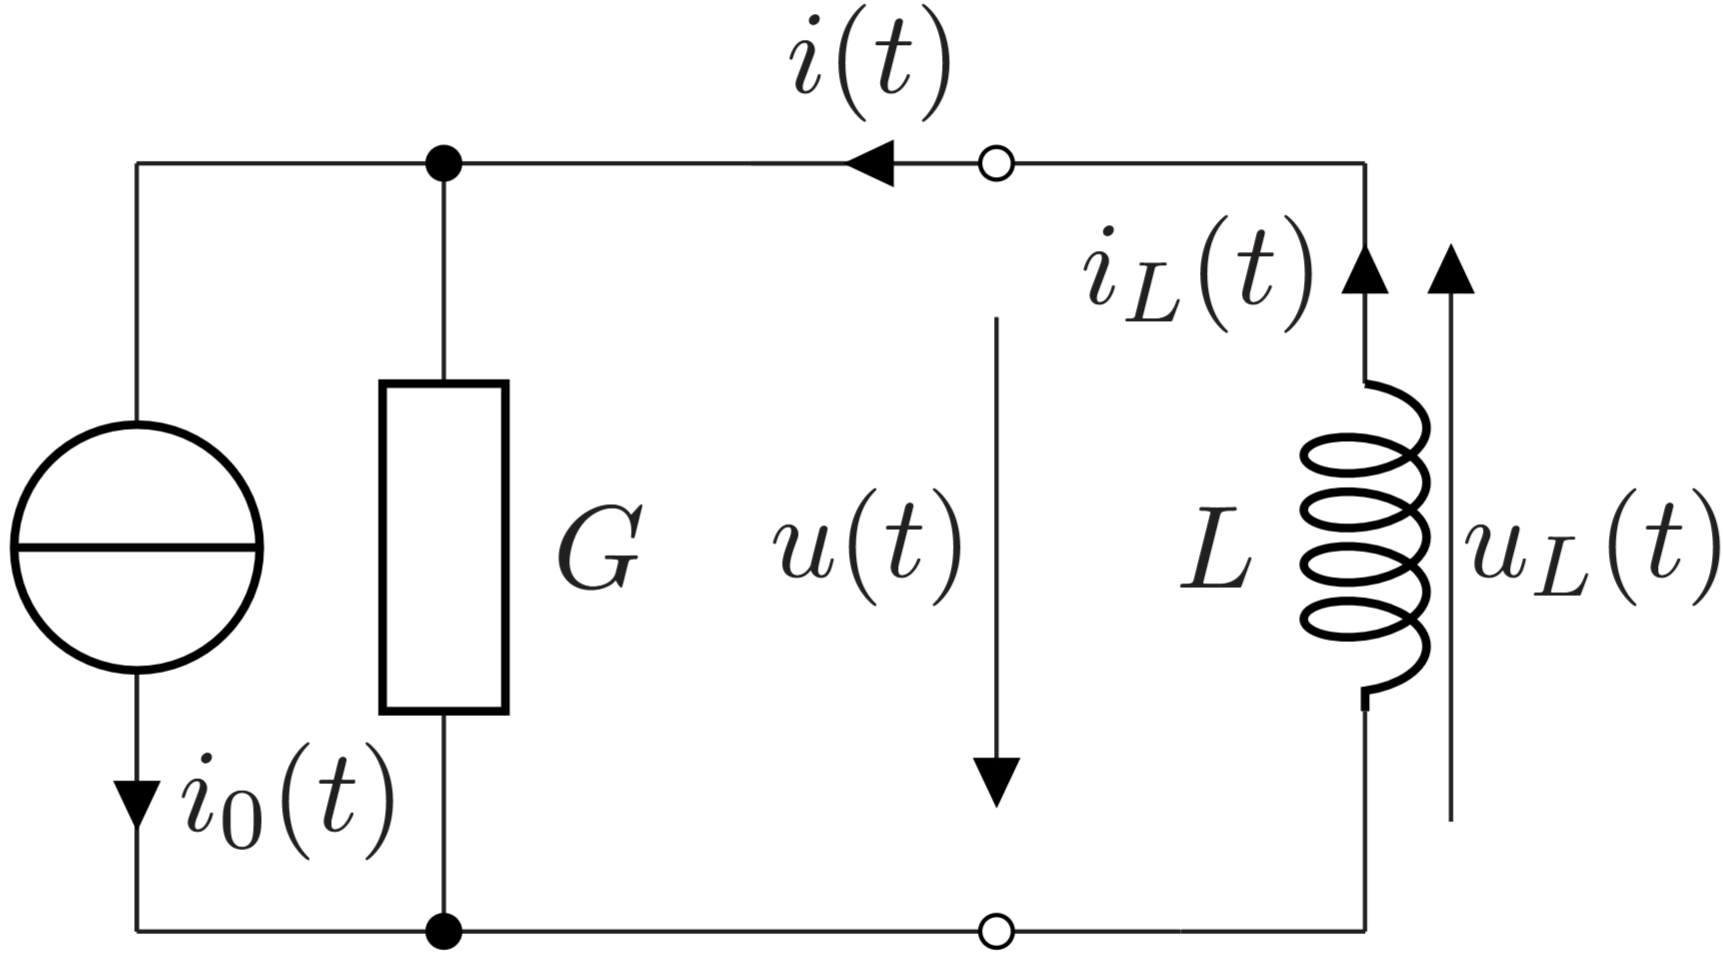
\includegraphics[width=.35\linewidth]{img/mayer-norton}\\
            Zustandsgröße & $x(t) = u_C(t)$ & $x(t) = i_L(t)$\\
            Zeitkonstante & $\tau = RC$ & $\tau = GL$\\
            \brule
        \end{tabular*}
    }

    \textbf{II. Aufstellen DGL} (kanonische Form)\\
    $\dot x(t) = - \fr{1}{\tau}x(t) + \fr{1}{\tau}v(t)$ mit der Erregung $v(t)$\\
    \textbf{III. Lösen der DGL}\\
    Konstante Erregung:  $x(t) = \overbrace{x_\infty}^{\text{GGP}} + (x_0 - x_\infty )\e^{-\frac{t-t_0}{\tau}}$ \\
    Allgemeine Erregung: $x(t) = \underbrace{x_0\e^{-\frac{t-t_0}{\tau}}}_{\text{zero-input-response}}+\underbrace{\int_{t_0}^t{\frac{1}{\tau}v(t')\e^{-\frac{t-t'}{\tau}}}}_{\text{zero-state-response}}$ \\
    mit $u_{C,\infty}=U_0$ bzw. $i_{L,\infty}=I_0$\\
    \textbf{IV. Dynamischer Pfad}\\
    \tablebox{
        \begin{tabular*}{\columnwidth}{@{\extracolsep\fill}ll@{}} \trule
            Kapazität & Induktivität\\ \mrule
            $u=u_C, i=-i_C$ & $u=-u_L, i=i_L$ \\ \mrule
            $i < 0$: $u$ wird größer & $u < 0$: $i$ wird größer\\
            $i > 0$: $u$ wird kleiner & $u > 0$: $i$ wird kleiner\\
            $i = 0$: GGP & $u = 0$: GGP\\
            \brule
        \end{tabular*}
    }
    \textbf{Toter Punkt:} kein GGP, aber Pfad kann nicht fortgesetzt werden \ra Sprung der nicht stetigen Größe ($i_C$ oder $u_L$)\\
    \textbf{Gleichgewichtspunkt (GGP):}\\
    Punkt der Kennlinie im u-i-Diagramm, wo $i_C$ bzw. $u_L$ gleich 0 sind. Daraus folgt $\dot u_C=0$ bzw. $\dot i_L=0$ \\
    \begin{tabular*}{\columnwidth}{@{\extracolsep\fill}ll@{}}
        Kapazität & Induktivität\\ \mrule
        $\dot u_F = 0 \ra i_F = 0$ & $\dot i_F = 0 \ra u_F = 0$\\
        \mrule
    \end{tabular*}
    \begin{itemize}
        \item[a)] stabil, falls der Pfad zum GGP konvergiert/im GGP ist
        \item[b)] instabil, falls sich der Pfad vom GGP wegbewegt
        \item[c)] virtuell, falls der Pfad in einen toten Punkt auf dem verlängertem Pfad auf der Achse läuft
    \end{itemize}
    }

    \subsection{Stabile Schaltung ($\tau > 0$)}
    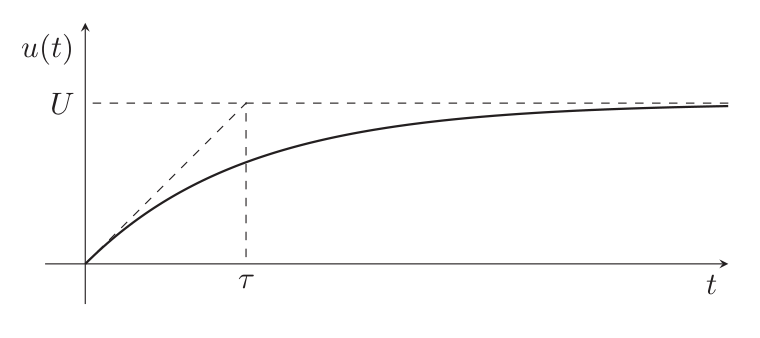
\includegraphics[width=.8\linewidth]{img/graph-stabil}
    \subsection{Instabile Schaltung ($\tau < 0$)}
    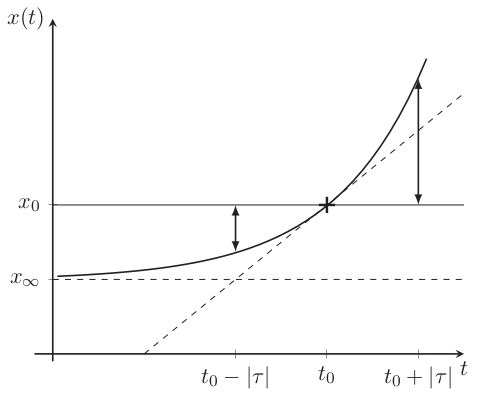
\includegraphics[width=.8\linewidth]{img/graph-instabil}
    \subsection{Dynamischer Pfad}
    %TODO Dynamischer Pfad S.24


    \subsection{Sprung- und Impulsantwort}\label{sec:Sprung- und Impulsantwort}

    \subsubsection{Sprungantwort}
    Sprungfunktion: $\sigma(t) = \begin{cases}1 & \text{für } t > 0 \\ 0 & \text{für } t < 0\end{cases}$\\
    Sprungantwort: $x_\sigma(t) = (1 - \exp{(-\fr{t}{\tau})})\sigma(t)$

    \subsubsection{Impulsantwort}
    rechteckförmiger Signalverlauf der Erregung. Erregung wird kurz eingeschaltet und dann wieder ausgeschaltet.\\
    Erregung: $p_\Delta(t)=\begin{cases}
            \frac{1}{\Delta} & 0 \le t < \Delta \\
            0                & \text{sonst}
        \end{cases}$ \\

    Impulsantwort: $\tau h_\Delta(t)=\tau\begin{cases}
            0                                                                      & t < 0            \\
            \frac{1}{\Delta}(1-e^{-\frac{t}{\tau}})                                & 0 \le t < \Delta \\
            \frac{1}{\Delta}(1-e^{-\frac{\Delta}{\tau}})e^{-\frac{t-\Delta}{\tau}} & t \ge \Delta
        \end{cases}$

    \begin{center}
        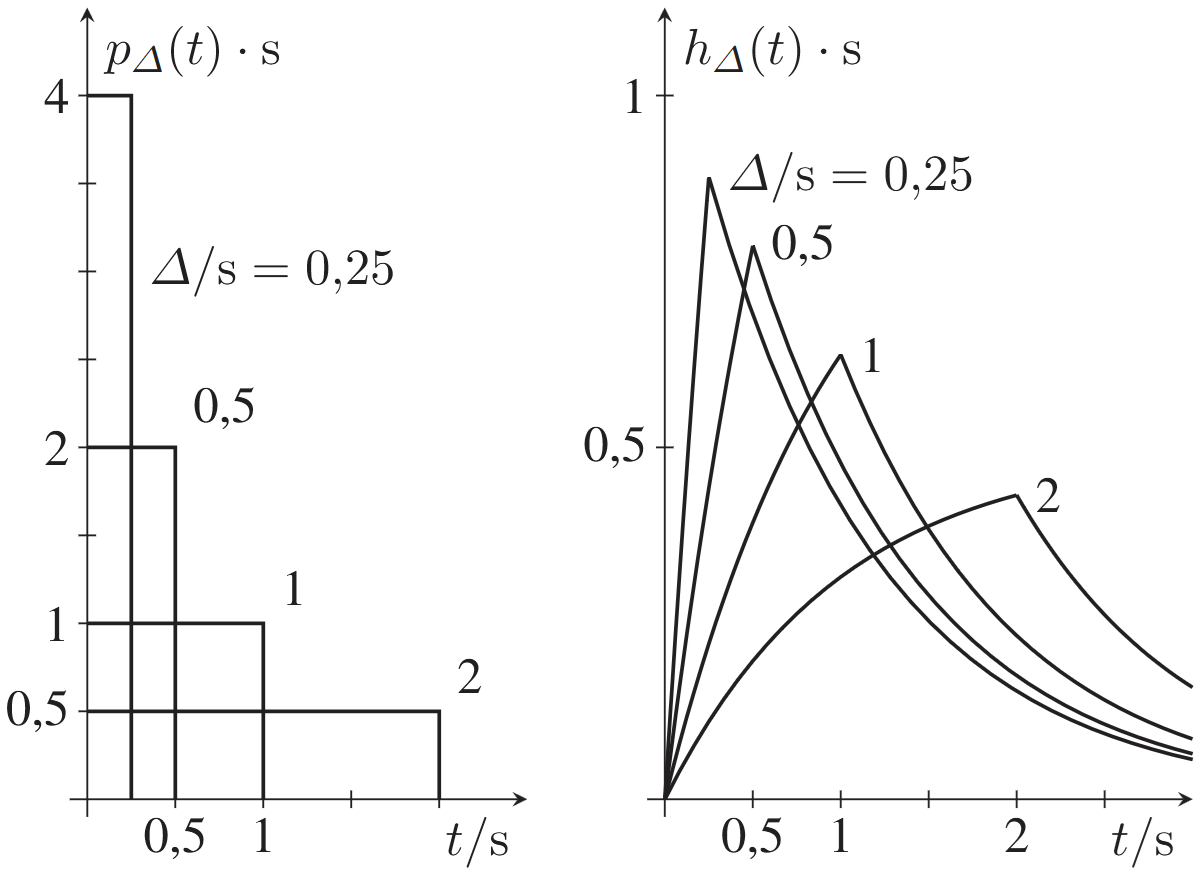
\includegraphics[width=.8\linewidth]{img/sprungantwort_impulsantwort}
    \end{center}

    \textbf{Grenzübergang $\Delta \rightarrow 0$} \\
    Erregung (Einheitsimpuls): $\delta(t)=0$ für $t\ne 0$ und $\int_{-\infty}^\infty \delta(t)\mathrm dt=1$\\
    Impulsantwort: $h(t)=\frac{1}{\tau}e^{-\frac{t}{\tau}}\sigma(t)=\frac{\mathrm d x_\sigma(t)}{\mathrm dt}$
    \begin{center}
        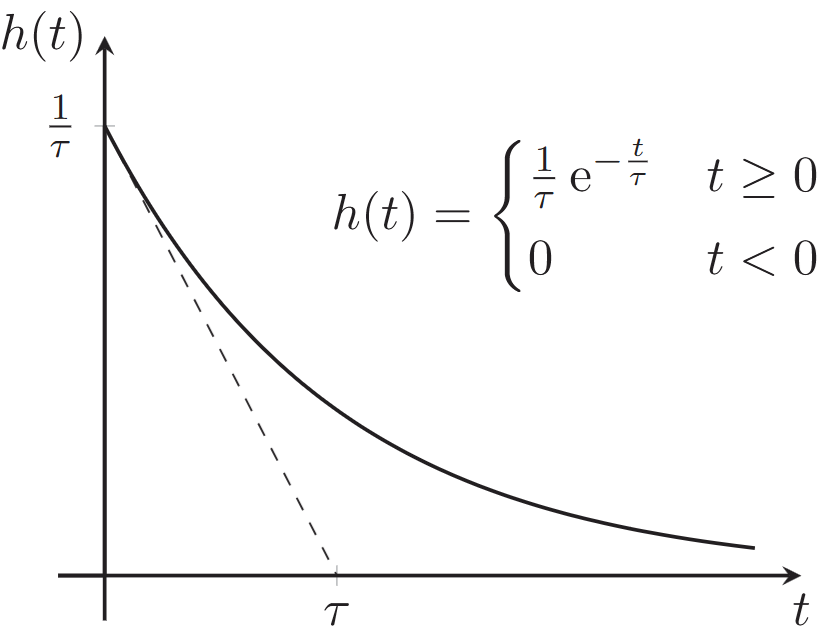
\includegraphics[width=.5\linewidth]{img/impulsantwort.png}
    \end{center}

    \subsection{Sprungphänomene}
    Tritt auf, falls Pfad in einen toten Punkt läuft.\\
    Führt zu einer sprungartigen Fortsetzung des dynamischen Pfades auf einem anderen Kennlinienast (Stetigkeitsregel beachten).\\
    Beispiele: Relaxationsoszilator, astabiler Multivibrator

    \subsection{Populationswachstum}
    Zustandsgröße Population $p(t)$, DGL $\dot p(t)=\alpha p(t)=-\frac{1}{\tau} p(t) \Rightarrow \tau < 0 \Rightarrow $ System instabil \\
    Lösung: $p(t)=p_0e^{\alpha(t-t_0)}$

    \subsection{Marktgleichgewicht}
    Zustandgröße Preis $p(t)$, DGL:
    \begin{align*}
        \dot p(t)=m(\underbrace{\gamma -\delta p(t)}_{\text{Nachfrage } d(t)} - \underbrace{(\alpha p(t)-\beta)}_{\text{Angebot } s(t)})= \\
        \underbrace{-(m\delta + m\alpha)}_{-\frac{1}{\tau}<0 \Rightarrow \tau > 0}p(t)+m\gamma+m\beta                                     \\
        \alpha,\beta,\gamma,\delta,m > 0
    \end{align*}
    $\Rightarrow$ System stabil \\
    Lösung: $p(t)=\frac{\gamma + \beta}{\delta + \alpha} + (p_0 - \frac{\gamma + \beta}{\delta + \alpha})e^{-(m\delta +m\alpha)(t-t_0)}$

    %TODO Sprungphänomene S.26

    %TODO Solow-Swan-Modell S.35
    \section{Systeme zweiten Grades}
    \subsection{Differentialgleichungssystem aufstellen}
    \textbf{I. Schaltung umzeichnen}\\
    Zeichne die Schaltung so um, dass beide Reaktanzen an den äußeren Seiten sind.\\
    \textbf{II. Matrix aufstellen}
    (Quellen vernachlässigen)
    \begin{itemize}
        \item[a)] zwei Kapazitäten: Leitwertsmatrix $\ma G$
        \item[b)] zwei Induktivitäten: Widerstandsmatrix $\ma R$
        \item[c)] Kapazität (Tor 1) und Induktivität (Tor 2): Inverse Hybridmatrix $\ma{H'}$
        \item[d)] Induktivität (Tor 1) und Kapazität (Tor 2): Hybridmatrix $\ma{H}$
    \end{itemize}

    \textbf{III. Quellenvektor aufstellen}

    \textbf{IV. Differentialgleichungssystem aufstellen}
    \subsection{Phasenportraits}
    \subsubsection{Zeichnen des Phasenportraits}
    \textbf{I. Bestimmung der Eigenwerte $\lambda_i$ und Eigenvektoren $q_i$}\\
    $\lambda_{1,2} = \frac{tr(\ma A)}{2} \pm \sqrt{\frac{tr(\ma A)^2}{4}-det(\ma A)}$\\
    $a_{12} \neq 0 \Rightarrow \mathbf{q}_i = \begin{bmatrix}-a_{12}\\a_{11}-\lambda_i\end{bmatrix}$\quad $a_{21} \neq 0 \Rightarrow \mathbf{q}_i = \begin{bmatrix}a_{22}-\lambda_i\\-a_{21}\end{bmatrix}$\quad$a_{12} = a_{21} = 0 \Rightarrow \mathbf{q}_1 = \begin{bmatrix}1\\0\end{bmatrix}, \mathbf{q}_2 = \begin{bmatrix}0\\1\end{bmatrix}$\\
    Falls Eigenvektoren komplex: $\mathbf{q}_r = \Re{q_1}$\qquad$\mathbf{q}_i = \Im{q_1}$\\
    \textbf{II. Bestimmung des Fixpunktes}\\
    $\mathbf{A}\mathbf{x}_\infty + \mathbf{B}\mathbf{v} = 0 \Rightarrow \mathbf{x}_\infty = -\mathbf{A}^{-1} \mathbf{B}\mathbf{v}$\\
    \textbf{III. Art des Phasenportraits}\\
    \textbf{Strudelpunkt}\\
    $\lambda_{1/2} = \alpha \pm \beta j$, $\alpha \neq 0$: Je nach $\sgn(\alpha)$ (in-)stabiler Strudel in Drehrichtung von $\mathbf{q}_r$ ($\xi_{\text{reel}1}$) nach $-\mathbf{q}_i$ ($\xi_{\text{reel}2}$)\\
    
\includegraphics[width=.7\linewidth]{phase-strudel}\\
    \textbf{Wirbelpunkt}\\
    $\lambda_{1/2} = \pm \beta j$: Wirbel in Drehrichtung von $\mathbf{q}_r$ ($\xi_{\text{reel}1}$) nach $-\mathbf{q}_i$ ($\xi_{\text{reel}2}$)\\
    
\includegraphics[width=.7\linewidth]{phase-wirbel}\\
    \textbf{Knotenpunkt}\\
    $\lambda_{1,2} < 0, |\lambda_1| < |\lambda_2|$: Trajektorien von Richtung (Eigenvektor) des schnelleren Eigenwerts ($\mathbf{q}_2, \xi_2$) schmiegen sich an an Richtung des langsameren Eigenwerts ($\mathbf{q}_1, \xi_1$).\\
    
\includegraphics[width=.7\linewidth]{phase-knoten}\\ \\
    \textbf{Sattelpunkt}\\
    $\lambda_1 < 0 < \lambda_2 $: Zwei Geraden in Eigenrichtungen, von stabiler Richtung zu GGP, zu instabiler Richtung. Restliche Trajektorien Hyperbeln mit Geraden als Asymptoten.\\
    
\includegraphics[width=.7\linewidth]{phase-sattel}\\
    \textbf{IV. Einzeichnen von Fixpunkt und Eigenvektoren}\\
    Die Eigenvektoren werden ausgehend vom Fixpunkt eingezeichnet. Bei konjugierten Eigenvektoren zeichnet man den Realteil und den negierten Imaginärteil.\\
    \subsubsection{Isokline}
    Kurve, auf der die Steigung der Trajektorie konstant ist.\\
    $m = \frac{\dot{x}_2}{\dot{x}_1}$, falls $m = 0: \dot{x}_2 = 0$ bzw. $m = \infty: \dot{x}_1 = 0$
    \subsubsection{Separatrix}
    Kurve, die Gebiete mit verschiedenem Langzeitverhalten trennt.
    \subsection{Lösung der Zustandsgleichungen}
    \subsubsection{Homogener Fall}
    Transformation autonom (konst. Erregung) $\Rightarrow$ homogener Fall mit: $\ \mathbf{x}' = \mathbf{x} - \mathbf{x}_\infty$.\\ \\
    $\lambda_1 \neq \lambda_2$: $\mathbf{x}(t) = \ c_1\e^{\lambda_1 t}\mathbf{q}_1 + c_2\e^{\lambda_2 t}\mathbf{q}_2$\\
    $\lambda_1 = \lambda_2 = \lambda$: $\mathbf{x}(t) = e^{\lambda t}(\mathbf{1} + (\mathbf{A} -\lambda \mathbf{1})t) [\mathbf{q}_1 \ \mathbf{q}_2]^T$\\
    komplexe Eigenwerte: $c_1 \e^{\alpha t}(\cos{(\beta t)}\mathbf{q}_{\text{reell}} - \sin{(\beta t)}\mathbf{q}_{\text{imag}}) + c_2\e^{\alpha t}(\sin{(\beta t)}\mathbf{q}_{\text{reell}} - \cos{(\beta t)}\mathbf{q}_{\text{imag}})$\\
    \subsubsection{Transformation auf Normalform}
    Gegeben: $\dot{x} = \mathbf{A} x$\\
    Normalgleichung: $\dot{\xi} = \Lambda \xi$\\
    Eigenwerte $\lambda_1, \lambda_2$ und Eigenvektoren $\mathbf{q}_1, \mathbf{q}_2$ berechnen\\
    $\mathbf{Q} =  \begin{bmatrix} \mathbf{q}_1 & \mathbf{q}_2 \end{bmatrix}$\\
    $\Lambda = \mathbf{Q}^{-1}\mathbf{A}\mathbf{Q} = \begin{bmatrix} \lambda_1 & 0 \\ 0 & \lambda_2 \end{bmatrix}, \xi = \mathbf{Q}^{-1} x$\\
    $x(t) = \mathbf{Q} \xi(t) = \mathbf{Q} \exp(\Lambda(t-t_0))\mathbf{Q}^{-1} x_0$\\
    \subsubsection{Transformation auf Jordan-Normalform}
    Gegeben: $\lambda = \lambda_1 = \lambda_2, \mathbf{A}$ ist keine Diagonalmatrix\\
    $J = \begin{bmatrix} \lambda & 1 \\ 0 & \lambda \end{bmatrix}, \mathbf{Q}' = \begin{bmatrix} \mathbf{q}_1' & \mathbf{q}_2' \end{bmatrix}, \xi'(t) = \mathbf{Q}'^{-1}\mathbf{x}(t)$\\
    Zustandsgleichung in Jordan-Normalform: $\dot{\xi}'(t) = \mathbf{J} \xi'(t)$\\
    Lösung der Zustandsgleichung:\\ $\xi'(t) = \begin{bmatrix} \exp(\lambda(t-t_0))\xi_1'(t_0)+(t-t_0)\exp(\lambda(t-t_0))\xi_2'(t_0) \\ \exp(\lambda(t-t_0))\xi_2'(t_0) \end{bmatrix}$\\
    Rücktransformation: $\mathbf{x}(t) = \mathbf{Q}'\xi'(t) = \mathbf{q}_1'\xi_1'(t) + \mathbf{q}_2'\xi_2'(t)$\\
    \subsubsection{Transformation auf reellwertige Normalform}
    Gegeben: $\lambda_{1/2} = \alpha \pm \beta j, \mathbf{q}_r, \mathbf{q}_i$\\
    $\Lambda_\text{reell} =  \begin{bmatrix} \alpha & - \beta \\ \beta & \alpha \end{bmatrix}$\\
    $\mathbf{Q}_\text{reell} = \begin{bmatrix} \mathbf{q}_r & - \mathbf{q}_i \end{bmatrix}$\\
    $\mathbf{x}_\text{reell} = \mathbf{Q}_\text{reell}^{-1} \e^{\Delta t}\mathbf{Q}_\text{reell}$\\
    $\dot{\xi}_\text{reell} (t) = \Lambda_\text{reell}\xi_\text{reell}(t)$\\
    \subsection{Zeitverlauf der Zustandsvariablen}
    Eigenwerte: $\lambda_i = \alpha + j\beta$ mit Dämpfung $\alpha$ und Schwingung $\beta$\\
    \textbf{Stabilität:} stabil, falls $\alpha < 0$, sonst instabil\\
    Schwingung mit Kreisfrequenz $\omega = \beta$\\
    \tablebox{
        \begin{tabular*}{\columnwidth}{l@{\extracolsep\fill}|l} \ctrule
            Fall & Schwingungsart \\ \cmrule
            $\alpha = 0, \beta \neq 0$ & ungedämpfte Schwingung\\
            $\alpha < 0, \beta \neq 0$ & schwach gedämpfte Schwingung\\
            $\lambda_1 = \lambda_2 < 0, \beta = 0$ & aperiodischer Grenzfall\\
            $\lambda_1 \neq \lambda_2, \beta = 0$ & stark gedämpfte Schwingung\\ \cbrule
        \end{tabular*}
    }
    \subsection{Sprung- und Impulsantwort (analog zu \ref{sec:Sprung- und Impulsantwort})}
    Zustandsgleichung der Form $\dot{\mathbf{x}}(t) = \mathbf{A}\mathbf{x}(t)+\mathbf{b}v(t)$.\\
    Ausgangsgleichung der Form $y(t) = \mathbf{c}^T\mathbf{x}(t) + dv(t)$.
    \subsubsection{Sprungantwort}

    Sprungantwort \\$y_\sigma(t) = (d-\mathbf{c}^T\mathbf{A}^{-1}\mathbf{b})\sigma (t) + \mathbf{c}^T\mathbf{A}^{-1}\exp{(\mathbf{A}t)}\mathbf{b}\sigma(t)$ \\
        mit der Sprungfunktion $\sigma(t)$\\ \\
        Für ein stabiles System mit $\lim_{t\rightarrow\infty}\exp{(\mathbf{A}t)} = \mathbf{0}$ ($\lambda_{\text{real}} < 0$) konvergiert die Sprungantwort wie folgt: $y_{\sigma,\infty} = d + \mathbf{c}^T\mathbf{A}^{-1}\mathbf{b}$.
        \subsubsection{Impulsantwort}
    $h(t) = \frac{d}{dt} y_\sigma(t)$\\
    $h(t) = d\delta (t) + \mathbf{c}^T\exp{(\mathbf{A}t)}\mathbf{b}\sigma(t)$
        \subsection{Steady-State- und Transientenantwort}
    $\mathbf{x}(t) = \mathbf{x}_{\text{trans}}(t) + \mathbf{x}_{\text{steady}}(t)$
        \subsubsection{Steady-State-Antwort}
    $\mathbf{x}_{\text{steady}}(t) = \text{Re}\{Y(j\omega)\e^{j\omega t}\}$\\
    $X_{\text{steady}}(t) = H(j\omega) \cdot U_{\text{in}}$
        \subsubsection{Transientenantwort}
        Die Summe der Polstellen von $H(j\omega)$ ist die Transientenantwort.\\
    $\mathbf{x}_{\text{trans}}(t) = \exp{(\mathbf{A}t)} \cdot \mathbf{x}_{\text{trans}}(t)$
        \section{Nichtlineare dynamische Systeme}
        \begin{enumerate}
            \item Alle Fixpunkte bestimmen $\mathbf{f}(x_\infty) \stackrel{!}{=} \mathbf{0}$
            \item Jacobimatrix bestimmen
            \item Fixpunkte in Jacobimatrix einsetzen und Eigenwerte und Eigenvektoren bestimmen
            \item Überprüfen des \textbf{Satzes von Hartmann/Grobmann}: \\Für alle Eigenwerte gilt $\Re{\lambda_i} \neq 0$
            \item Phasenportrait zeichnen (lokale Phasenportraits stetig verbinden)
        \end{enumerate}
        \subsection{Energiefunktion}
        Eigenschaften: stetig, lokal nicht konstant, auf jeder Trajektorie konstant\\
        Schaltung ist \textbf{konservativ}, falls:\\
    $\dot{E} = 0 \Leftrightarrow \frac{\partial E(\mathbf{x})}{\partial x_1} \dot{x}_1 + \frac{\partial E(\mathbf{x})}{\partial x_2} \dot{x}_2 + \hdots + \frac{\partial E(\mathbf{x})}{\partial x_n} \dot{x}_n = 0$\\
        Erweiterung des Satzes von Hartmann/Grobmann: Jacobimatrix hat nur imaginäre Eigenwerte und Schaltung ist konservativ $\Leftrightarrow$ GGP ist Wirbelpunkt
        \subsection{Oszillatoren}
        Schaltung mit periodischem Verlauf der Zustandsgrößen\\
        Voraussetzung: nichtlinear, nur ein Fixpunkt (instabil)\\
        \textbf{Van der Pol-Oszillator:}\\
        \parbox{.5\linewidth}{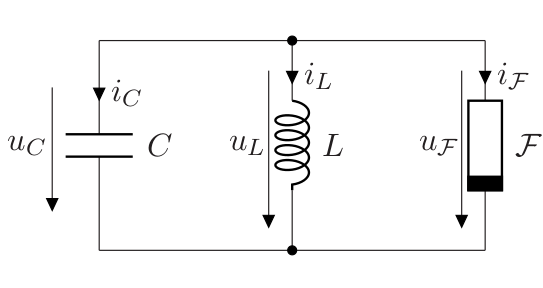
\includegraphics[width=\linewidth]{img/van-der-pol}}
        \parbox{.5\linewidth}{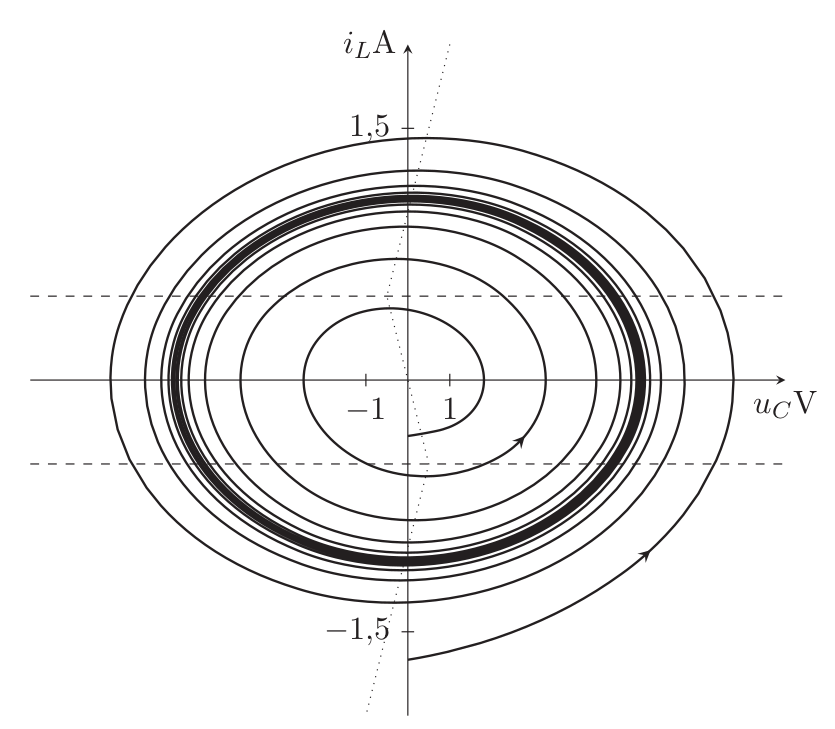
\includegraphics[width=\linewidth]{img/fast-harmonischer-oszillator}}\\
        \textbf{Relaxationsoszillator:}\\
        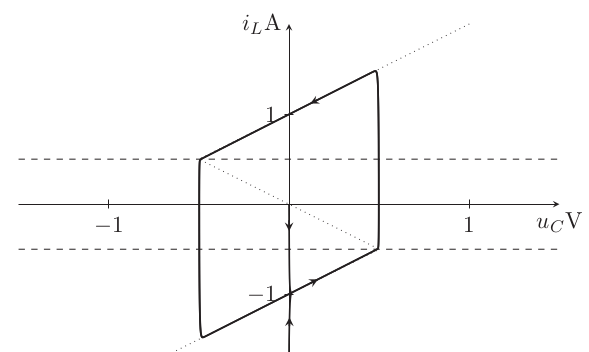
\includegraphics[width=.5\linewidth]{img/relaxationsoszillator}
        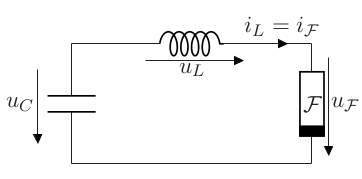
\includegraphics[width=.5\linewidth]{img/relaxationsoszillator-schaltung}
        \section{Dynamische Schaltungen beliebigen Grades}
        \subsection{Verallgemeinerte Zustandsgleichungen}
    $\frac{d}{dt} \begin{bmatrix}\mathbf{0} & \mathbf{0}\\\mathbf{0} & \mathbf{0}\\\mathbf{M}_1 & \mathbf{N}_1\end{bmatrix}\begin{bmatrix}\mathbf{u}\\\mathbf{i}\end{bmatrix} = - \begin{bmatrix} \mathbf{B} & \mathbf{0} \\ \mathbf{0} & \mathbf{A} \\ \mathbf{M}_0 & \mathbf{N}_0\end{bmatrix}\begin{bmatrix}\mathbf{u}\\\mathbf{i}\end{bmatrix} + \begin{bmatrix}\mathbf{0}\\\mathbf{0}\\\mathbf{e}\end{bmatrix}$\\
    $\mathbf{M}_1, \mathbf{N}_1$: Elementgleichungen der reaktiven Elemente\\
    $\mathbf{M}_0, \mathbf{N}_0$: Elementgleichungen aus Tableau\\
    $\mathbf{B}$: KVL, $\mathbf{A}$: KCL\\
        ($e = 0 \Leftrightarrow$ keine Quellen enthalten)
        \section{Analyse dynamischer Systeme im Frequenzbereich}
        \subsection{Laplace-Transformation}
        Für kausale Funktionen mit $f(t) = 0$ für $t < 0$:\\
    $F(p) = \mathcal L\{f(t)\} = \int_0^\infty f(t) \e^{-pt}dt$\\
        Rücktransformation: \\
    $f(t) = \mathcal L^{-1}\{F(p)\} = \fr{1}{2\pi j}\int_{\gamma-j\infty}^{\gamma+j\infty} F(p) \e^{-pt}dt$\\
        \subsubsection{Rechenregeln}
        \begin{itemize}
            \item Linearität: $\mathcal L\{\alpha f(t) + \beta g(t)\} = \alpha F(p) + \beta G(p)$
            \item Differentiationssatz: $\mathcal L\{\dot f(t)\} = pF(p) - f(0)$
            \item Faltung: $\mathcal L\{(a * b)(t)\} = A(p)B(p)$
        \end{itemize}
        \subsubsection{Wichtige Laplace-Transformationen}
        \begin{itemize}
            \item $\mathcal L\{\alpha\e^{\beta t}\} = \fr{\alpha}{p-\beta}$
            \item $\mathcal L\{\e^{\ma At}\} = \fr{1}{p\ma 1 - \ma A}$
        \end{itemize}
        Allgemeine Lösung im Frequenzraum:\\
    $x(p) = \fr{1}{p\ma 1-\ma A}x_0 + \fr{1}{p\ma 1-\ma A}bV(p)$\\
    $x(t) = x(0)\e^{\ma At} + \int_0^t \e^{\ma A(t-t')}v(t')b dt'$
        \subsection{Übertragungsfunktion}
    $H(j\omega ) = \fr{\text{Ausgang}}{\text{Eingang}}$\\
        Nullstellen des Ausgangs werden als $p_{0,i}$ bezeichnet\\
        Nullstellen des Eingangs werden als \textbf{Eigenfrequenzen} $p_{\infty,i}$ bezeichnet\\
        Polstellen $p_{\infty, i}$ von $H(j\omega)$ sind die Eigenwerte der Systemmatrix\\
        \textbf{Bestimmung der Differentialgleichung:}\\
    $H(\j\omega) = \frac{U_A}{U_E} = \frac{a_0 + a_1 \j\omega + a_2 (\j\omega)^2}{e_0 + e_1 \j\omega + e_2 (\j\omega)^2}$\\
    $U_A (e_0 + e_1 \j\omega + e_2 (\j\omega)^2) = U_E  (a_0 + a_1 \j\omega + a_2 (\j\omega)^2)$\\
    $e_0 u_a(t) + e_1 \dot{u}_a(t) + e_2 \ddot{u}_a(t) = a_0 u_e(t) + e_1 \dot{u}_e(t) + e_2 \ddot{u}_e(t)$\\
        3dB-\textbf{Grenzfrequenz:} $\abs{H(j\omega)}^2 = \fr{1}{2}$\\
        \textbf{Stabilität:} Re$\{p_{\infty,i}\} < 0$ \quad $\forall i$\\
        Darstellung einer Schaltung in Abhängigkeit der Frequenz\\
    $H(j\omega) = \abs{H(j\omega)} \exp (j\angle H(j\omega))$\\
    $\phi (\omega) = \angle H(j\omega) = \begin{cases}
        \arctan\frac{\text{Im}\{H(j\omega)\}}{\text{Re}\{H(j\omega)\}}     & $für $\text{Re}\{H(j\omega)\} \geq 0 \\
        \arctan\frac{\text{Im}\{H(j\omega)\}}{\text{Re}\{H(j\omega)\}}+\pi & $für $\text{Re}\{H(j\omega)\} < 0    \\
    \end{cases}$\\
        logarithmierte Darstellung des Betrages: $v(\omega) = 20 \log_{10} \abs{H(j\omega)}$\\
        \subsection{Bodediagramm}
        %TODO Graph, verschiedene Typen (siehe Tut Teutsch)
        \begin{enumerate}
            \item Übertragungsfunktion faktorisieren\\
                  $H(jw) = K \cdot \prod_{n=1}^n \left(x_n+\frac{jw}{w_n}\right)^{z_n}$\qquad$z_n \in \mathbb{Z} \ \{0\}$\\
            \item Logarithmierte Beträge der einzelnen Faktoren aufstellen\\
                  \quad a) Konstanter Faktor: $y = 20\cdot\log_{10}(K)$dB\\
                  \quad b) Falls $x_n = 0$: Gerade durch $(\omega_n, 0$dB$)$\\
                  \quad c) Falls $z_n < 0$: Bis $\omega_n$ Funktion gleich 0dB, dann linear um $20 \cdot\log_{10}(x_n)$dB pro Dekade fallend\\
                  \quad d) Falls $z_n > 0$: Bis $\omega_n$ Funktion gleich 0dB, dann linear um $20 \cdot\log_{10}(x_n)$dB pro Dekade steigend\\
            \item Phase der Faktoren bestimmen
            \item Logarithmierte Beträge und Phasen aufaddieren
            \item Separates Zeichnen des Betrages $v(\omega)$ und der Phase $\phi(\omega)$ in zwei Diagramme
        \end{enumerate}
        \subsection{Ortskurve}
        \begin{enumerate}
            \item Bestimmung von diversen Werten der Übertragungsfunktion
            \item Eintragen in der komplexen Ebene
            \item Punkte stetig verbinden
        \end{enumerate}
        \parbox{.6\linewidth}{
            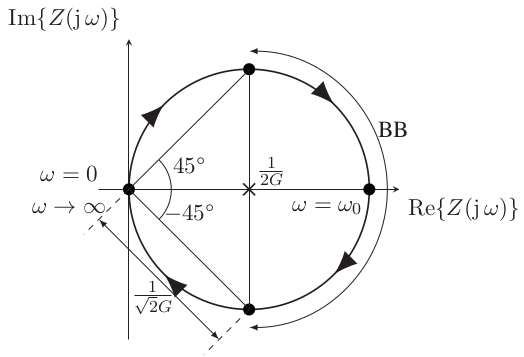
\includegraphics[width=\linewidth]{img/ortskurve-r}}
        \parbox{.4\linewidth}{
            Hier: Widerstandsortskurve eines Parallelschwingkreises. Kann auch Leitwert oder eine andere Übertragungsfunktion sein}
        \subsection{Filtertypen}
        \textbf{Hochpass:} $|H(j0)| = 0, |H(j\omega)| \rightarrow c \text{ für } \omega \rightarrow \infty$\\
        \textbf{Tiefpass:} $|H(j0)| = c, |H(j\omega)| \rightarrow 0 \text{ für } \omega \rightarrow \infty$\\
        \textbf{Bandpass:} $|H(j0)| = 0, |H(j\omega)| \rightarrow 0 \text{ für } \omega \rightarrow \infty, |H(jw_0)| = c$\\
        \textbf{Bandsperre:} $|H(j0)| = c, |H(j\omega)| \rightarrow c \text{ für } \omega \rightarrow \infty, |H(jw_0)| = 0$\\
        \textbf{Allpass:} $|H(j0)| = c$ (Phase kann sich trotzdem abhängig von $\omega$ ändern!)\\
        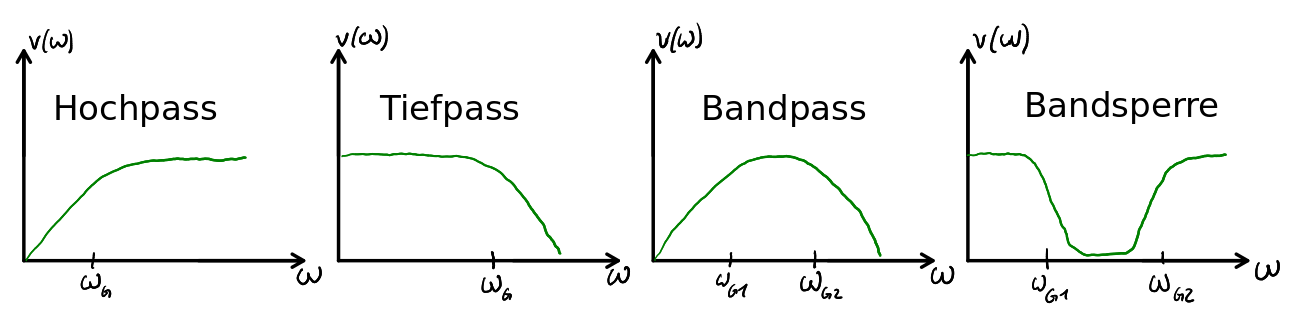
\includegraphics[width=\linewidth]{img/filtertypen}
        \subsection{Schwingkreis}
        Resonanzfrequenz: $\omega_0 = \sqrt{\frac{1}{LC}}$\\
        Gütefaktor: $Q = \frac{\omega_0C}{G} = \frac{1}{\omega_0LG} = \frac{\sqrt{C}}{G\sqrt{L}}$\\
        Eigenfrequenzen: $p_{\infty,1,2} = -\frac{\omega_0}{2Q}\pm \frac{\omega_0}{2Q}\sqrt{1-4Q^2}$
    \section{SPICE}
    \renewcommand{\t}{\texttt}
    \subsection{Bauteile}
    \begin{itemize}
        \item \t{L<Name> <Knoten1> <Knoten2> <Wert>}: Spule zwischen Knoten \t{<Knoten1>} und Knoten \t{<Knoten2>} mit Induktivität \t{<Wert>}
        \item \t{C<Name> <Knoten1> <Knoten2> <Wert>}: Kondensator zwischen Knoten \t{<Knoten1>} und Knoten \t{<Knoten2>} mit Kapazität \t{<Wert>}
        \item \t{R<Name> <Knoten1> <Knoten2> <Wert>}: Widerstand zwischen Knoten \t{<Knoten1>} und Knoten \t{<Knoten2>} mit Widerstandswert \t{<Wert>}
        \item \t{U<Name> <Knoten1> <Knoten2> <Wert>}: Spannungsquelle zwischen Knoten \t{<Knoten1>} und Knoten \t{<Knoten2>} mit Spannung \t{<Wert>} (Spannung positiv bei \t{<Knoten1>})
        \item \t{I<Name> <Knoten1> <Knoten2> <Wert>}: Stromquelle zwischen Knoten \t{<Knoten1>} und Knoten \t{<Knoten2>} mit Stromstärke \t{<Wert>} (Strom in Richtung \t{<Knoten2>})
    \end{itemize}
    \subsection{Parameterbefehle}
    \begin{itemize}
        \item \t{.step param <Param> <Start> <End> <Step>}: Alle Parameter \t{\{<Param>\}} werden vom Startwert \t{<Start>} bis \t{<End>} während der Simulation als Treppenfunktion mit Schrittweite \t{<Step>} eingesetzt.
        \item \t{.step param <Param> list <Wert1> <Wert2> ...}: Simulation wird $n$ mal für jeden Parameterwert durchgeführt.
        \item \t{.step oct param <Param> <Start> <End> <StepsPerOct>}
    \end{itemize}
    \subsection{Analysearten}
    \begin{itemize}
        \item \t{.tran <Endtime>}: Transientenanalyse im Zeitbereich von $t = 0$ bis $t = \text{\t{<Endtime>}}$. Bsp.: \t{.trans 60us}
    \end{itemize}

    \section{Simulink}
    TODO %TODO





    % Ende der Spalten
\end{multicols*}

\label{LastPage}

% Dokumentende
% ======================================================================
\end{document}